\chapter{Next generation detectors}
\label{CHAP::VERITAS}

%##############################################################################
%#                                                                            #
%#                   CHAPTER X : NEXT GENERATION DETECTORS                    #
%#                                                                            #
%##############################################################################

\label{SEC::VERITAS::INTRO}
%##############################################################################
%#             SECTION 0 : INTODUCTION TO NEXT GENERATION DETECTORS           #
%##############################################################################

The success of the current generation of ground-based detectors in the
300\,GeV to 10\,TeV energy range has motivated the construction of a
next generation of experiments. The design of these next generation
VHE \Gray detectors is guided by the desire to improve the flux
sensitivity over this range of energies and to reach lower energies
where there will be overlap with the energy range accessible to
upcoming satellite based experiments. Increased sensitivity will be
achieved by increasing the number of \Grays collected and improving
the discrimination of \Grays from background cosmic-rays.

The former is achieved by having larger light collection area, the
ultimate being to collect all of the light from the air shower with a
detector whose mirror area is comparable to the size of the \Cerenkov
light pool on the ground. The amount of light recorded from an air
shower increases more quickly with mirror area ($\propto$\,A) than the
fluctuations in the background light recorded from the night sky
($\propto$\,A$^{1/2}$), the principal background determining the
triggering threshold. Collecting more light allows this threshold to
be lowered and hence lower energy events to be collected. Two large
area detector designs have been adopted, the first employs a large
steerable telescope, exemplified by the MAGIC telescope
\citep{REF::LORENZ::1996NUCPHYSB} being built on La Palma which is a
17\,m carbon-fiber frame telescope with a 234\,m$^2$ mirror area. The
second are converted solar furnace experiments such as STACEE in New
Mexico \citep{REF::COVAULT::2001HAMBURG} and CELESTE
\citep{REF::CELESTE::1996PROPOSAL} in the French Pyrenees, which
comprise large fields of heliostats with area $\sim$2400\,m$^2$ and a
central light collecting tower which houses secondary optics and the
photon detectors. All of the upcoming experiments have, at minimum,
$75$\,m$^2$ of mirror area, equivalent to a 10\,m diameter dish.

Inability to discriminate \Grays from background cosmic-rays, cosmic
electrons and local muons is ultimately the factor that limits the
sensitivity of all ground-based experiments. The ability of a system
to discriminate between a \Gray signal and background events depends
on many factors, from the design of the instrument and the analysis
technique. Some of these factors can change during the lifetime of the
experiment, e.g.\ improved analysis algorithms, upgraded photon
detectors etc. It is the design of the instrument itself that
contributes, in the largest degree, to the elimination of background
events. An instrument that is designed to take advantage of the
inherent difference between signal events and background events can
achieve good intrinsic discrimination by its very nature. One such
design is an array of multiple telescopes viewing the air shower
stereoscopically from different points on the ground. Signals from
multiple telescopes, placed close enough that they all lie within the
\Cerenkov light pool of an air shower, can be combined in such a way
that \Grayc-like events produce a very different signal from
cosmic-ray events. The array can be triggered in a fashion that
eliminates local muon events and reduced accidental night-sky
triggers. Examples of such systems are VERITAS
\citep{REF::WEEKES::AP2002}, a system of seven 12\,m telescopes
in southern Arizona, which will be the largest array in the northern
hemisphere. HESS \citep{REF::HESS::2002BOOKLET} an array of four 12\,m
telescopes being built in Namibia and CANGAROO
\citep{REF::ENOMOTO::APP} a four, 10\,m telescope array in Australia will
survey the sources in the skies of the southern hemisphere. The array
technique has been successfully demonstrated, albeit with small
telescopes, by the HEGRA collaboration \citep{REF::KONOPELKO::1999AP}.

\section{VERITAS}
\label{SEC::VERITAS::INSTRUMENT}
%##############################################################################
%#               SECTION 1 : PARAMETERS OF THE VERITAS INSTRUMENT             #
%##############################################################################

The VERITAS experiment, which began construction in 2002, will be an
array of seven 12\,m telescopes, located in southern Arizona, USA. The
seven f/1.0 telescopes will be situated at the vertices and center of
a regular hexagon of side 80\,m. The \Cerenkov light pool of \Gray
induced showers that impact close to the center of the array will
encompass all seven telescopes, each of which will have a different
view of the shower development which can be combined to give a more
accurate reconstruction of the properties of the primary than those
previously available to single telescope ground-based \Gray
instruments.

VERITAS will be built in three stages between 2002 and 2007. After a
single prototype telescope is completed in 2003 and operated for a
number of months, the second stage, a four telescope array will be
completed in 2005. The final stage, bringing the full seven telescope
array on-line, will then be completed in 2007. An evaluation of the
characteristics of the four telescope array is presented in detail in
this chapter.

\begin{figure}[t]
\begin{minipage}[c][0.27\textheight][c]{\textwidth}
\hspace*{\fill}
\resizebox{!}{0.27\textheight}{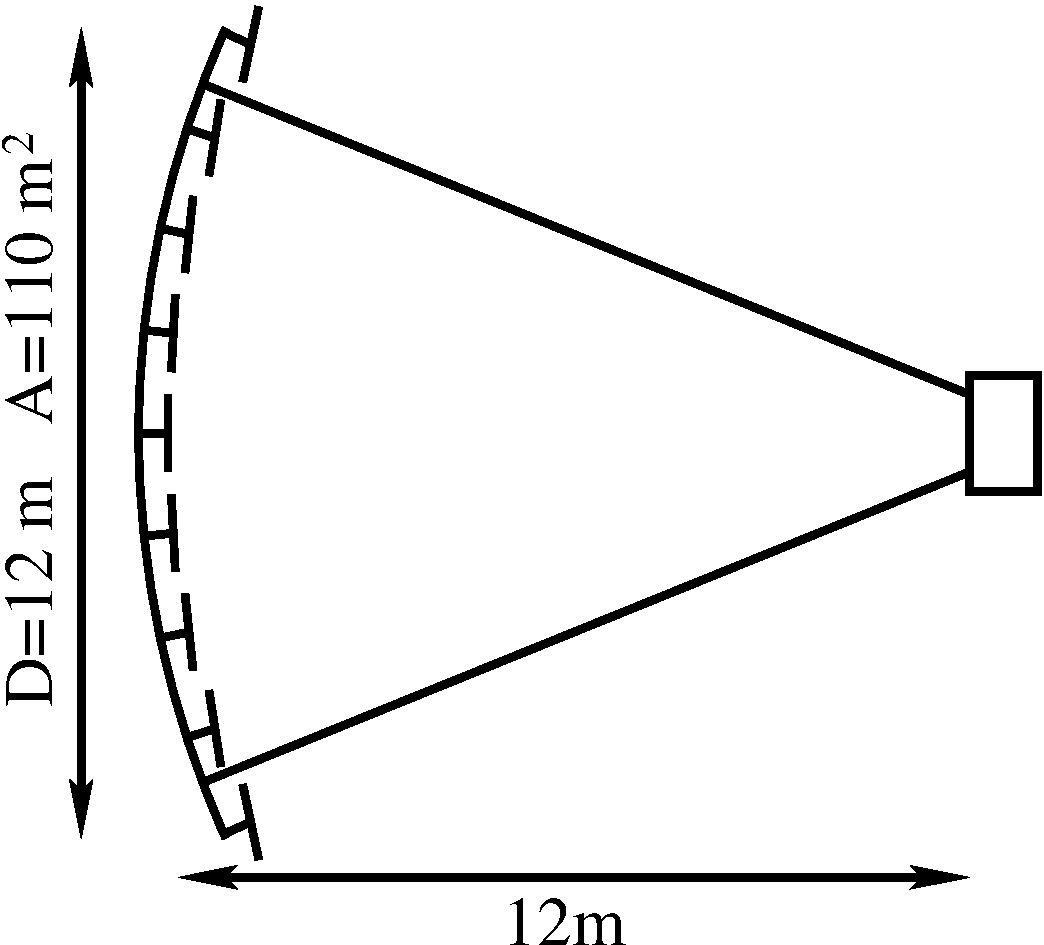
\includegraphics{plots/chap-veritas/vscope-base.pdf}}
\hspace*{\fill}
\resizebox{!}{0.27\textheight}{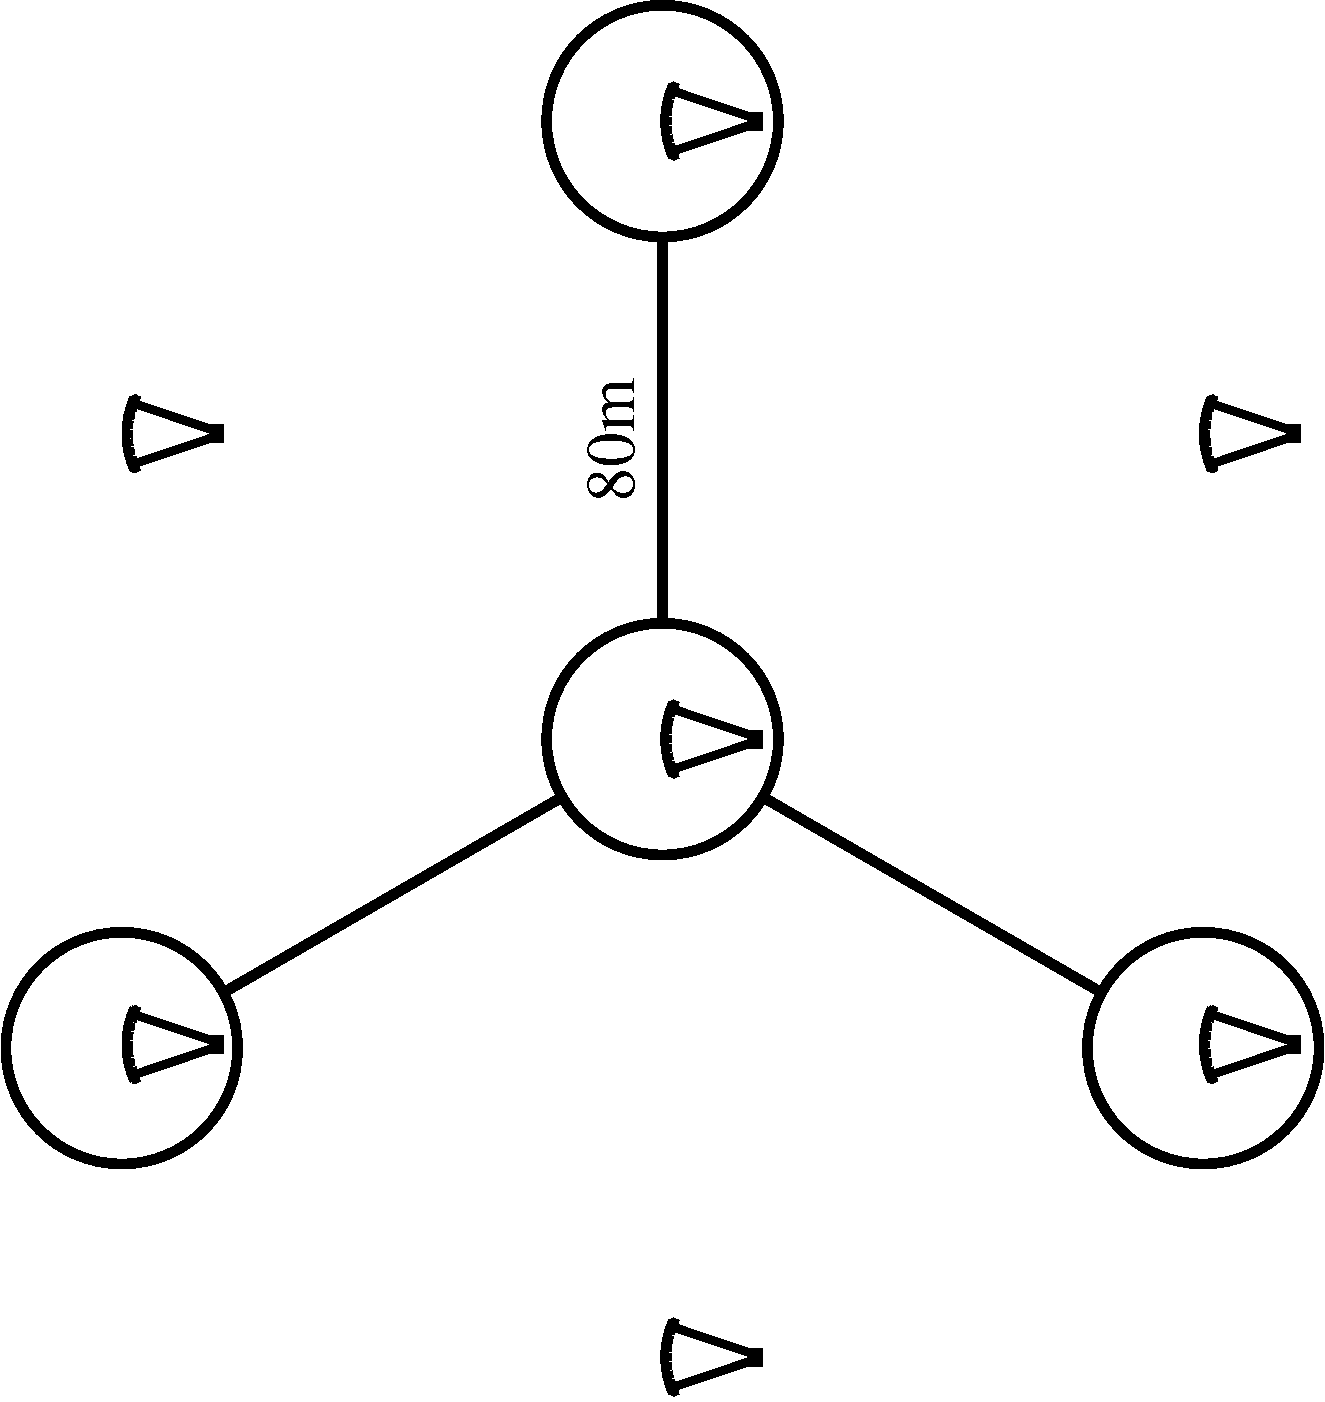
\includegraphics{plots/chap-veritas/varray-base.pdf}}
\hspace*{\fill}
\end{minipage}
\caption{\label{FIG::VERITAS::PHYSICAL} (Left) Dimensions of proposed 
VERITAS telescopes. (Right) Layout of seven telescope VERITAS array with 
\mbox{VERITAS-4} sub-array indicated.}
\end{figure}

\section{Overview of the VERITAS-7 simulations}
\label{SEC::VERITAS::V7SIMULATIONS}
%##############################################################################
%#             SECTION 2 : INTODUCTION TO VVVs VERITAS SIMULATIONS            #
%##############################################################################

\enlargethispage{14pt}
The results of a detailed simulation of the VERITAS array, as
performed by V.~Vassiliev, are presented in the original proposal by
the VERITAS collaboration to DOE and NSF
\citep{REF::VERITAS::1999PROPOSAL}. Two sub-array layouts were
simulated in detail, the complete system of seven 10\,m telescopes
separated by 80\,m and a sub-array of three telescopes separated by
80$\times\sqrt{3}\approx$140\,m.

In the time since this original work was performed, the proposed
design of the array has changed, the telescope diameter has been
increased to 12\,m and the initial configuration will be a 4 telescope
sub-array with an 80\,m separation. Each telescope will have 499
channels with a field of view of 3.5$^\circ$, as in the original
proposal. This chapter presents an extrapolation of the
characteristics of the four telescope array (VERITAS-4) from the
results of the original simulation. This was done by the author as
part of this dissertation; the details are presented in this
chapter. A brief overview of the original work is discussed first.

\subsection{Trigger conditions}
\label{SEC::VERITAS::V7TRIGGER}

The VERITAS system uses multi-level trigger hardware to eliminate much
of the accidental triggers, mostly due to the night-sky background
light. This allows the trigger level to be set as low as possible yet
keep the array trigger rate below 1\,kHz, as required by the data
acquisition system. The first level (L1), or ``channel-level'' trigger
is a discriminator set to trigger when the signal in the channel
exceeds a certain voltage, which is usually expressed in terms of a
number of photo-electrons (p.e.) detected within a certain time,
assuming a known single p.e.\ voltage pulse profile. The L2, or
``telescope-level'' trigger is a pattern recognition system which can
be programmed to require two, three or four neighboring channels
trigger in the camera within a certain coincidence time. This trigger
preferentially selects air-shower events over night-sky noise events
since the \Cerenkov light from an air-shower originates largely from
the same region of the sky, whereas night-sky fluctuations are
distributed randomly in the camera. The L3, or ``array-level'' trigger
is programmed to require that a certain number of telescope-level
triggers occur within a coincidence time. The L3 trigger is
responsible for initiating the data readout. The trigger requirements
used in the original VERITAS-7 simulations, for both the full array
and the three telescope sub-array, are listed in
table~\ref{TABLE::VERITAS::V7TRIGGER}.

\begin{table}[h]
\caption{\label{TABLE::VERITAS::V7TRIGGER}Trigger requirements for 
VERITAS-7 simulations.}
\centerline{\begin{tabular}{llll}\hline
(Sub-)Array & L1 trigger level & L2 (Telescope) & L3 (Array)\\\hline
Seven telescope array & 4.2 p.e. & 3 neighbors & 3 out of 7 (3/7) \\
Three telescope sub-array & 3.8 p.e. & 3 neighbors & 3 out of 3 (3/3)\\\hline
\end{tabular}}
\end{table}

\subsection{Reconstruction}
\label{SEC::VERITAS::V7RECONSTRUCTION}

Stereoscopic imaging of the air-shower with an array of imaging
telescopes allows the nature of the primary particle to be inferred
more accurately than with a single telescope. Reconstruction of the
parameters of a primary \Grayc, its energy, arrival direction and
impact parameter can be estimated by combining the images from the
individual telescopes.

The images of a compact air-shower, such as those from a \Gray
primary, tend to be aligned toward the arrival direction of the
primary. This tendency, when employed to a set of stereoscopic views
of an air-shower, allow the arrival direction to be determined by
overlapping the images from all telescopes and tracing the axes of the
individual images to a common point. For less compact showers, such as
those that are hadronic in origin, a single point of origin for all of
the images cannot usually be identified. In addition, by tracing the
axes of the images from their origin at the site of each telescope on
the ground, the location of the shower core impact with the ground can
be found. This simple geometrical reconstruction technique, as
illustrated in figure~\ref{FIG::VERITAS::SIMEVENT}, demonstrates the
the stereoscopic approach. Although this simple approach is powerful,
there are additional properties of the air-shower that can be inferred
from the images if a more sophisticated algorithm is adopted. One such
approach, described below, additionally provides an estimate of the
width of the shower emission region in space, a parameter that is
different for \Grayc- and background-induced events.

\begin{figure}[ht]
\hspace*{\fill}\resizebox{0.49\textwidth}{!}{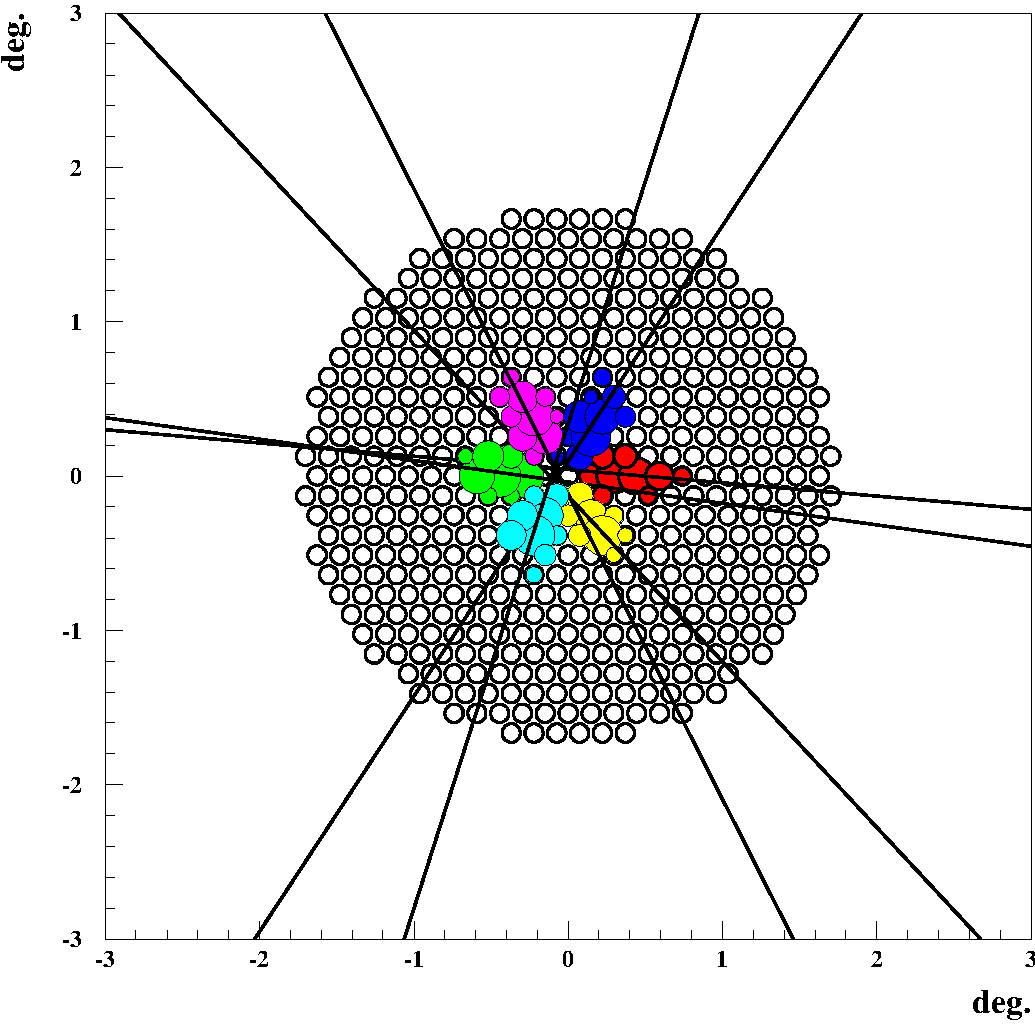
\includegraphics{plots/chap-veritas/recpicture1.pdf}}%
\resizebox{0.49\textwidth}{!}{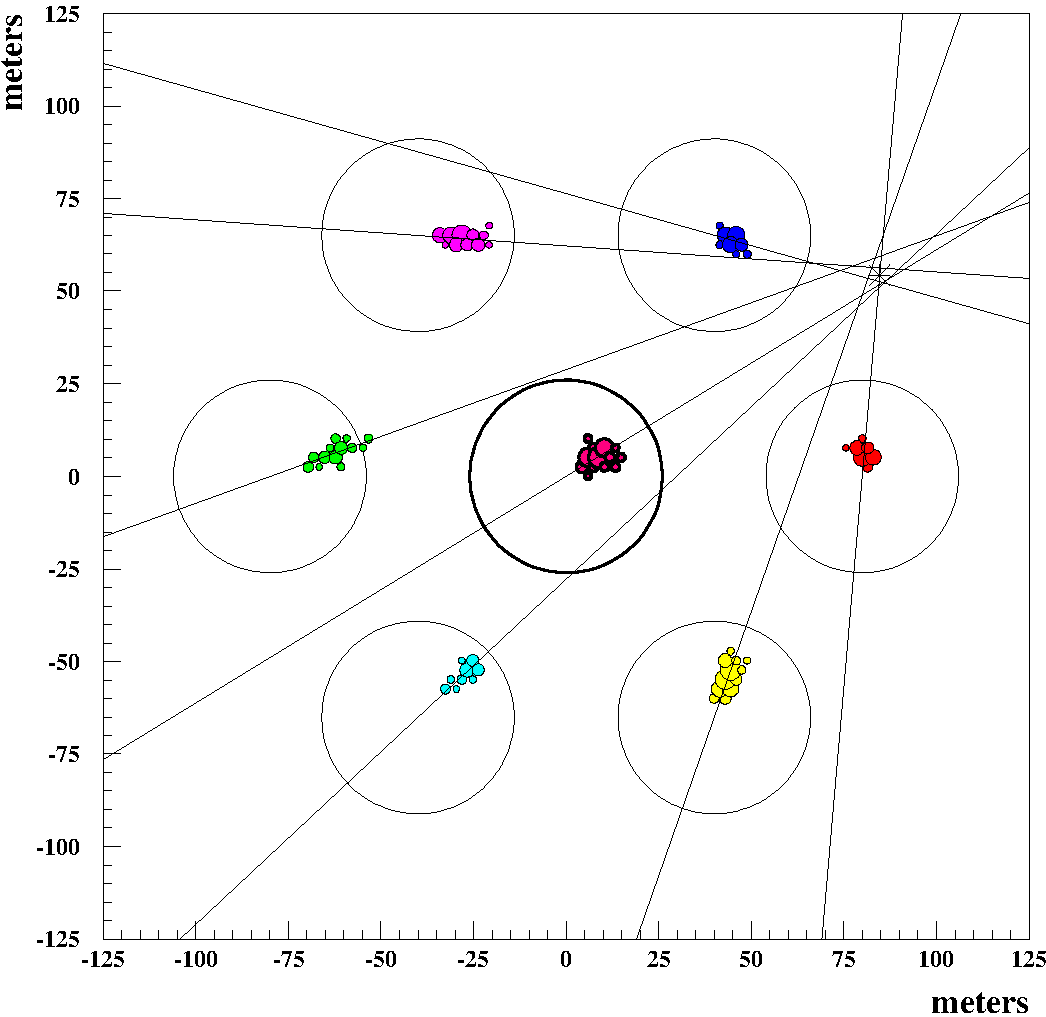
\includegraphics{plots/chap-veritas/recpicture2.pdf}}\hspace*{\fill}
\caption{\label{FIG::VERITAS::SIMEVENT} 
Simulated 300\,GeV \Gray events. (Left) The axes of the six images,
combined in \textit{angular space} in the field of view of the array,
point toward the origin of the \Grayc. (Right) Axes of the images,
when combined in \textit{2-D space} on the ground, indicate the impact
location of the shower core. From
\citet{REF::VERITAS::1999PROPOSAL}.}
\end{figure}

%The most likely origin of the \Gray is estimated by a least-squares
%approach. First, the images are conditioned as described in
%section~\ref{SEC::ANALYSIS::CONDITIONING}. For each channel that
%records a signal, an infinite number of rays are constructed, each
%reflected off a different part of the telescope mirror and out into
%space, giving the path of every possible \Cerenkov photon that could
%have ended up in the PMT. A model for the shower axis is then
%constructed using two parameters for shower direction ($\theta$,
%$\phi$) and two for the impact coordinates on the ground (x$_0$,
%y$_0$). For each ray, the minimum square distance, d$^2_i$, between
%the i'th ray and the shower axis is calculated. These squared
%distances are summed, weighted by the signal recorded in the
%appropriate channel, to give \mbox{$D^2$($\theta$, $\phi$, x$_0$,
%y$_0$)}, and the result minimized over all possible axis models. The
%axis parameters that minimize the total square distance is then taken
%as the best ``fit'' of the shower parameters to the data.

The most likely origin of the \Gray is estimated by a least-squares
approach. A simple model of the shower is constructed and the
parameters of the model adjusted to best fit the data from all
telescopes. It is assumed that the shower can be represented by an
``emission-region'' in the sky which is distributed around a
shower-axis, a line in 3-D space represented by two direction angles
($\theta$, $\phi$) and a shower impact location on the ground (x$_0$,
y$_0$). For convenience, $\theta$ and $\phi$ are taken as the
direction the shower-axis makes to the optical axis of the array,
figure~\ref{FIG::VERITAS::SHOWERAXISPARAM}. The impact location is
taken relative to the center of the array on the ground. As the shower
progresses through the atmosphere, \Cerenkov photons are emitted from
the emission region and these may be detected by the telescopes. The
density of \Cerenkov emission is proportional to the charged particle
density in the emission region. This region can be considered, to
first order, as an ellipsoid, symmetrically distributed around the
shower-axis with particular RMS width and length, the mean values of
which depend on the type of particle that initiated the shower and its
energy. Photons detected by a telescope will have taken an unknown
path from this region to the camera, having been reflected from some
portion of the telescope mirror. Ideally, one would like to
reconstruct the width of the emission-region, by tracing the detected
photons exactly back along their path in space, a process known as
back-propagation. It would then be possible to find the RMS width of
the emission region by calculating the mean square distance between
the photon paths and the shower axis. Of course, in reality this is
not possible for a number of reasons. First, it is not possible to
record every emitted photon, due to the limited telescope size and
inefficiencies in the detector, so any estimate will be statistical in
nature, with errors decreasing as the number of detected photons
increases. A more significant factor is the finite, non-zero size of
the PMTs in the focal plane. Since these detectors then subtend a
non-zero solid angle in space, there is inherent pixelation in the
arrival directions of the detected photons
(figure~\ref{FIG::VERITAS::RECONSTRUCTION3D}). Finally, it is
impossible to determine which portion of the 110\,m$^2$ mirror any
particular photon was reflected from. Essentially this means that no
single path through space can be assigned to any detected \Cerenkov
photon; an infinite number of possible paths must be considered.

\begin{figure}[p]
\centerline{\resizebox*{!}{0.3\textheight}{%
\resizebox*{!}{\textheight}{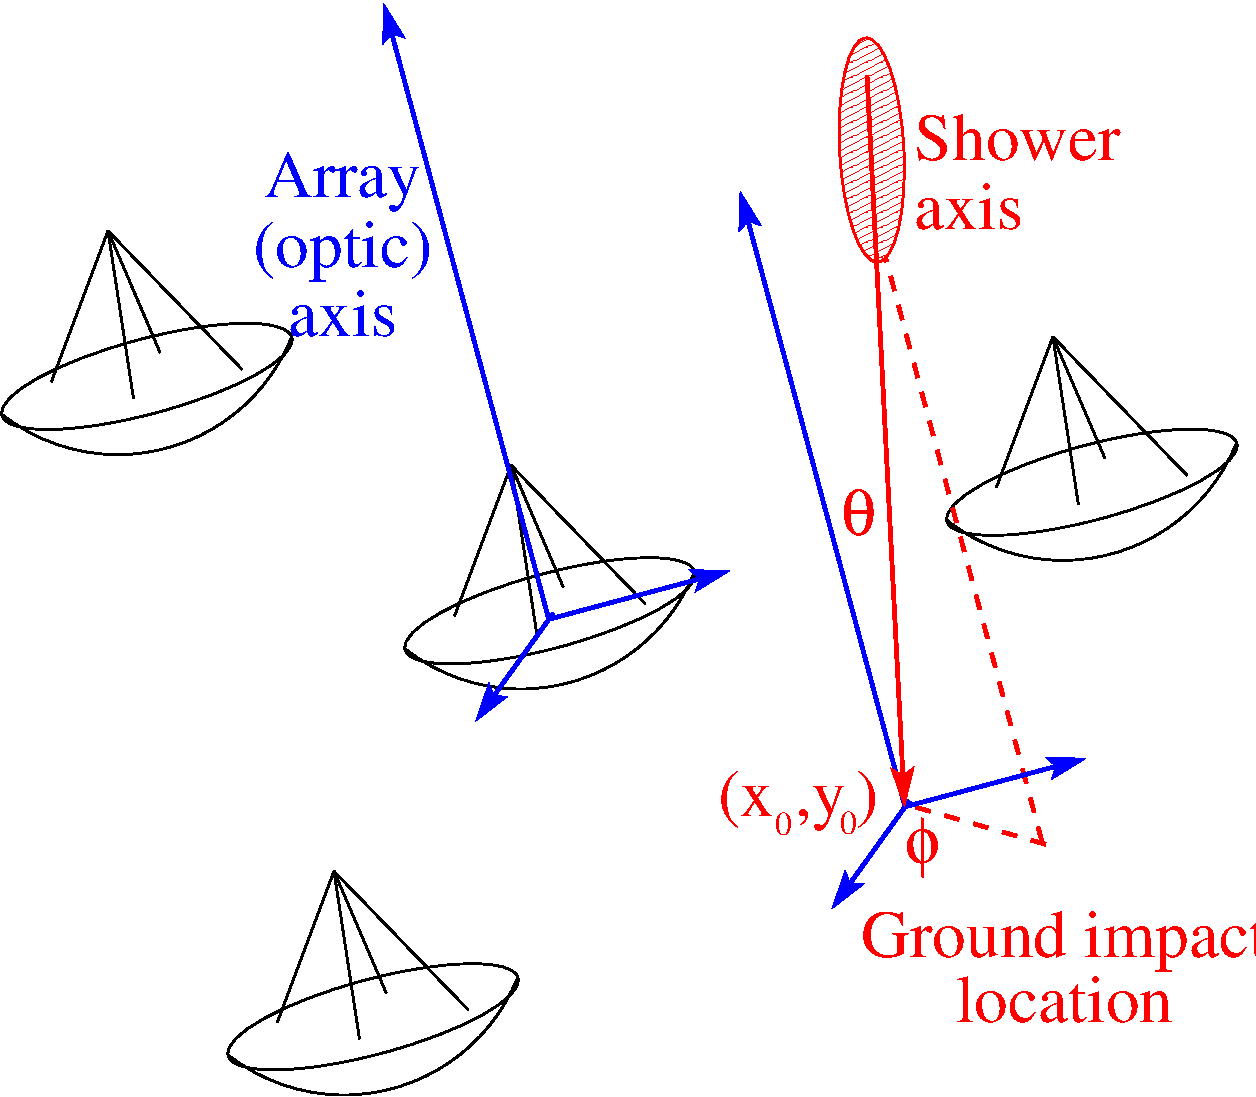
\includegraphics{plots/chap-veritas/vshower-param.pdf}}}}
\caption{\label{FIG::VERITAS::SHOWERAXISPARAM} Shower axis parameters, 
($\theta$, $\phi$) describe the direction of the reconstructed axis, 
(x$_0$, y$_0$) the point at which the axis intersects the ground.}
\end{figure}

\begin{figure}[p]
\hspace*{\fill}\resizebox*{!}{0.4\textheight}{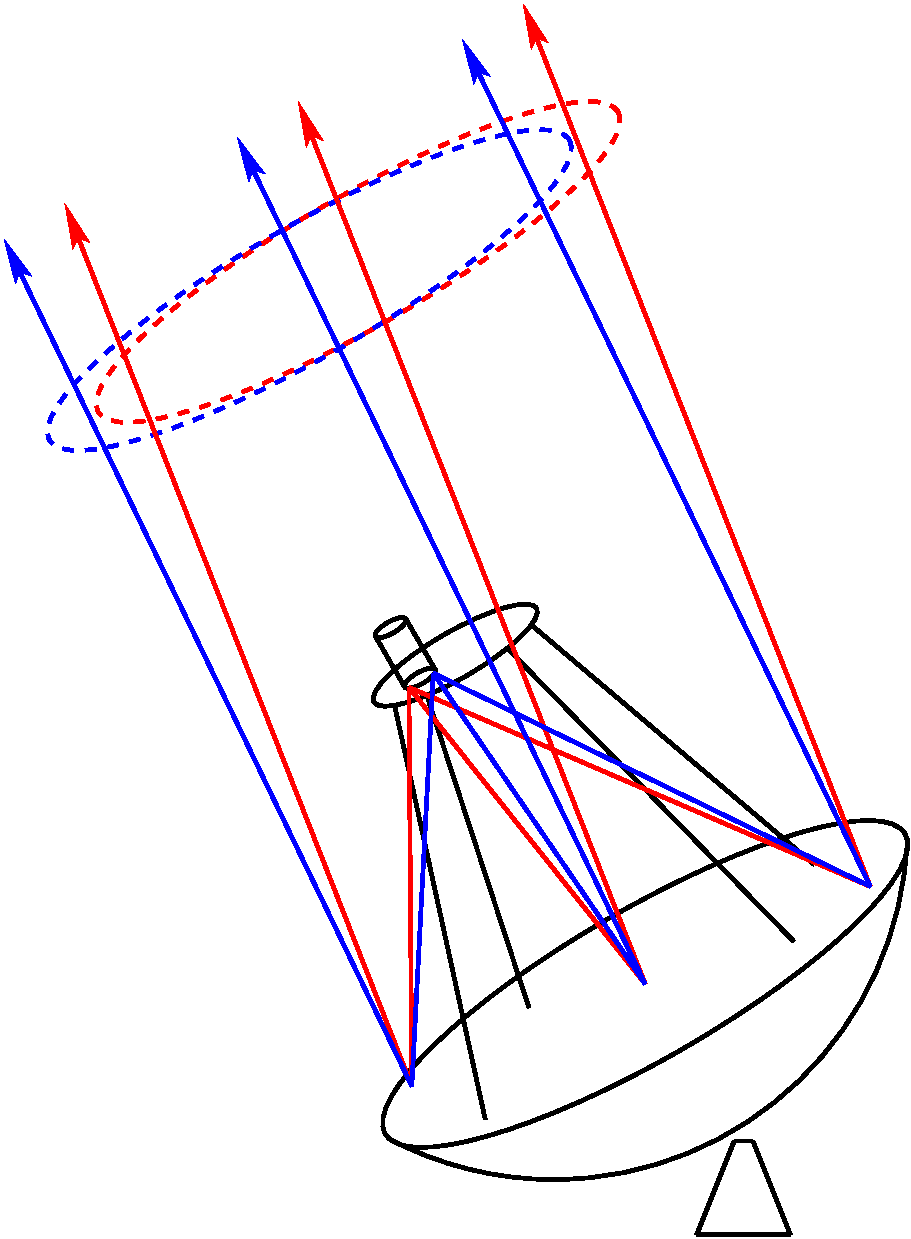
\includegraphics{plots/chap-veritas/vreconstruct2.pdf}}
\hspace*{\fill}\resizebox*{!}{0.4\textheight}{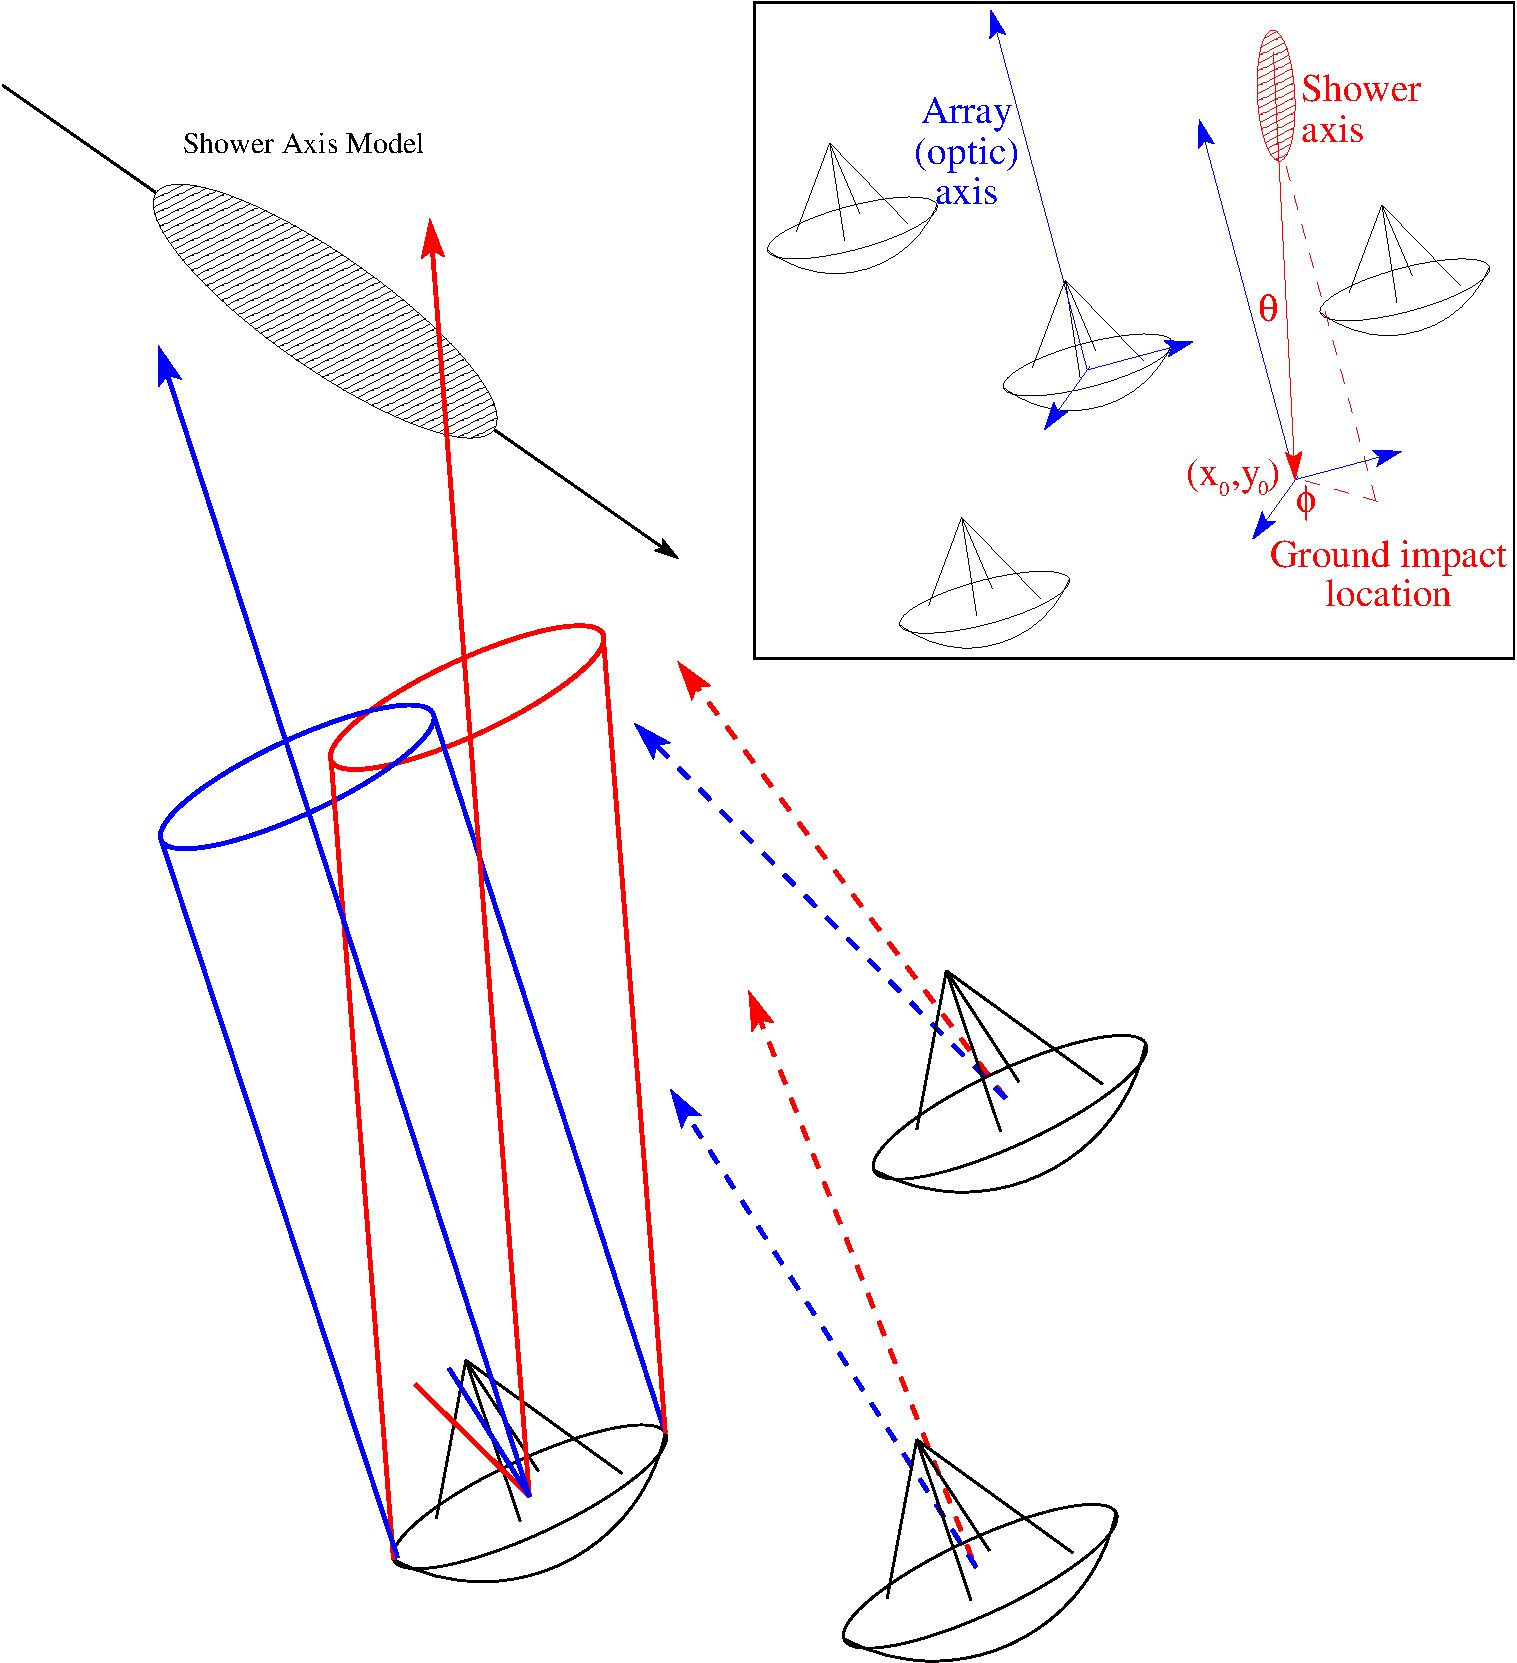
\includegraphics{plots/chap-veritas/vreconstruct-3d.pdf}}\hspace*{\fill}
\caption{\label{FIG::VERITAS::RECONSTRUCTION3D} (Left) Some of many 
possible paths for \Cerenkov photon detected in PMT. (Right) Shower
reconstruction technique. Detected photons are back-propagated from
PMT, reflected off the mirror and into space, illustrated as cylinders
projected from one of the telescopes.}
\end{figure}

Ideally, for each channel that records a signal, an infinite number of
back-propagated rays are constructed, each reflected off a different
part of the telescope mirror and propagated out into space, giving
every possible path for every \Cerenkov photon that was detected in
each of the PMTs. For each ray, the minimum square distance, d$^2_i$,
between the i'th ray and the shower axis is calculated. These squared
distances are summed to give \mbox{$D^2$($\theta$, $\phi$, x$_0$,
y$_0$)}, and the result minimized over all possible axis
parameters. Those parameters which minimize the total square distance
is then taken as the best ``fit'' of the shower-axis to the data,
since it requires an emission region with the smallest width. In
practice, an infinite number of back-projected rays are not
constructed for every PMT, a sample are used, distributed evenly over
the mirror area and over the area subtended in space by the PMT. The
actual value of $D_{\mathrm{min}}$, reflects the size of the emission
region but is also dependent on the PMT pixelation and mirror size.

\subsection{Background rejection}
\label{SEC::VERITAS::V7REJECTION}

Rejection of the isotropic cosmic-ray and cosmic-electron background
come from two separate selection techniques. The first, based on the
reconstructed arrival direction of the \Grayc, is applicable only to
point sources of {\Grayc}s, such as AGN and pulsar candidates. The
second, based on the ``shape'' of the air-shower is applicable to
point source and extended \Gray sources. In evaluating the performance
of the VERITAS array, only point source candidates are considered
here, for which the instrument will operate in its most sensitive
mode.

The goal of any selection technique is to eliminate as many background
events as possible while keeping as many of the \Grays as possible. It
is quite acceptable to eliminate up to $\sim$50\% of the \Grays in
order to have an efficient background ($>99.99\%$) rejection. In
general, the efficiency of background rejection is dependent on the
energy of the primary.  Showers resulting from high energy primaries
can be imaged accurately, allowing the primary to be identified with a
high degree of certainty. At these energies, background events can be
eliminated effectively. Low energy events are imaged less well,
identification of the primary is less certain and rejection is less
effective.

The first rejection technique, the ``aperture-cut'', exploits the fact
that, for a point source, only those events which are reconstructed as
having arrived from a point in space that lies close to the candidate
source need be considered. All other events can be rejected as part of
the isotropic background. Assuming the array is pointing directly at a
candidate \Gray source, the reconstructed shower axis parameter,
$\theta$, gives the distance between \Gray and the candidate
source. To reject a large part of the isotropic background it is
sufficient to define a maximum value, $\theta_{\mathrm{cut}}$, and
consider only events with $\theta<\theta_{\mathrm{cut}}$.

From simulations, it is found that the dispersion in the reconstructed
arrival direction of \Grays from a point source, depends on the energy
of the \Grayc. The instrument has a small dispersion for high energy
events, i.e.\ high energy events tend to be reconstructed as having
arrived from a small region of space surrounding their true
origin. The opposite is true for low energy events, which tend to be
reconstructed in a larger area surrounding the true origin.

The second rejection technique comes from consideration of the
physical meaning of
\mbox{$D_{\mathrm{min}}$($\theta$,$\phi$, x$_0$, y$_0$)}. $D$, the
RMS distance from the shower axis of the photons detected on the
ground, is related to the physical width of the \Cerenkov emission
region in space, and is generally larger for a hadronic shower than
for a compact \Gray shower, since the transverse momentum of an
average hadronic shower particle is larger in the former case, as
discussed in section~\ref{SEC::TECHNIQUE::SHOWERS}.

By simply choosing a ``shape-cut'', $D_{\mathrm{cut}}$ on the value
of $D_{\mathrm{min}}$ for a shower, one can preferentially keep
\Gray events, i.e.\ require that
$D_{\mathrm{min}}<$D$_{\mathrm{cut}}$. In practice, it is better
to make the cut a function of the primary photon energy,
$D_{\mathrm{cut}}$(E$_\gamma$). It is found that the rejection is
most efficient for very energetic \Grays and almost completely
ineffective for low energy {\Grayc}s.

To estimate the energy of the primary \Grayc, an ``energy estimator''
function, must be found. The estimator must relate the measured image
parameters, denoted as $\Theta=\{D, \theta, \phi, \mathrm{x}_0,
\mathrm{y}_0, \mathrm{S_i}, z\}$, where S$_\mathrm{i}$ is the signal 
recorded by the i'th telescope and $z$ is the angle between the zenith
and the axis of the array, to the energy of the primary. Many
approaches to energy estimation are possible. One approach is to find,
from simulations, an analytic function that estimates the average
amount of light collected in the array, given the energy of the
primary, the impact parameter,
\mbox{b=$\sqrt{\mathrm{x}_0^2+\mathrm{y}_0^2}$}, and the zenith
angle. This function can then be inverted to give an energy
estimator. Another approach is to determine the probability density
function $p(\Theta;\mathrm{E})$ describing the likelihood that the
observed parameters, $\Theta$, arose from an event of energy E. For
any given event, the probability density can be searched to give the
most likely energy of the particle. Energy estimation techniques
applicable to an array of telescopes are discussed in more detail in
\citet{REF::HOFMANN::1997KRUGER} and \citet{REF::AHARONIAN::1999AA342}.

Given an energy-estimator function, it is possible to calculate the
best value for the shape-cut, $D_{\mathrm{cut}}$(E$_\gamma$), and
aperture-cut, $\theta_{\mathrm{cut}}$(E), as a function of
energy. Since the shape-cut is applied to all data (from point- and
extended-sources), an optimum value is chosen for this function in the
absence of any aperture-cut. With these values chosen, optimum values
for the aperture-cut are chosen, with the shape-cut applied. This
process, originally done for the VERITAS-7 configuration, was repeated
for the VERITAS-4 evaluation and will be described in detail in
section~\ref{SEC::VERITAS::V4CUTS}.

\section{Performance of the four telescope VERITAS sub-array.}
\label{SEC::VERITAS::V4}
%##############################################################################
%#        SECTION 3 : MY WORK ON DERIVING THE VERITAS-4 CHARACTERISTICS       #
%##############################################################################

Evaluation of the VERITAS-4 sub-array was done by interpolation from
the full VERITAS-7 characteristics introduced above. This was done in
two steps, first the results of the original analysis for the 3/3;10m
(3 triggering out of an array of 3, 10\,m telescopes) and 3/7;10m
configurations were scaled from the original 10\,m diameter case to a
12\,m case. These scaled results are designated 3/3;12m and
3/7;12m. Finally an interpolation to the required 3/4;12m array was
made between the scaled 3/3;12m and 3/7;12m characteristics.

\subsection{Trigger level}
\label{SEC::VERITAS::V4TRIGGER}

At the time this work was performed, it was planned to locate the
VERITAS array under the dark skies of Montosa canyon in southern
Arizona. The mean background photon rate from the night sky was taken
to be, $\langle NSB_{\mathrm{flux}}\rangle$\,$\approx$
\,2--4$\times$10$^{12}$\,s$^{-1}$m$^{-2}$sr$^{-1}$,
the factor of two in range corresponding to the variation from a patch
of dark sky to the bright Galactic Plane region. For a telescope with
110\,m$^2$ mirror area and PMTs of angular diameter 0.15$^\circ$ in
the focal plane, and after factoring in the mirror reflectivity and
efficiency of the PMTs, this corresponds to a detected photon rate of
$\langle NSB 
\rangle$\,$\approx$\,0.16--0.32\,ns$^{-1}$\,channel$^{-1}$. The L2,
telescope-trigger coincidence time is taken to be 8\,ns., i.e., a
requirement that three neighboring channels to trigger within
8\,ns. The L3, array-trigger coincidence time is 40\,ns., i.e.\
requiring that three telescopes trigger within 40\,ns. Determining the
various trigger rates (L1, L2, L3) given the night-sky background rate
and given a L1 pixel trigger threshold requires that the response of
the various components of the trigger be simulated and subjected to
random, Poisson distributed, background photons. This was done by
J.~Hall from the Univerity of Utah, and the results are presented in
figure~\ref{FIG::VERITAS::NSB} for completeness. The rate of
triggering due to background cosmic ray events is also displayed; this
is discussed in more detail in section~\ref{SEC::VERITAS::V4CR}.

\begin{figure}[t]
\begin{minipage}{\textwidth}
\hspace*{\fill}
\resizebox{0.7\textwidth}{!}{\rotatebox{270}{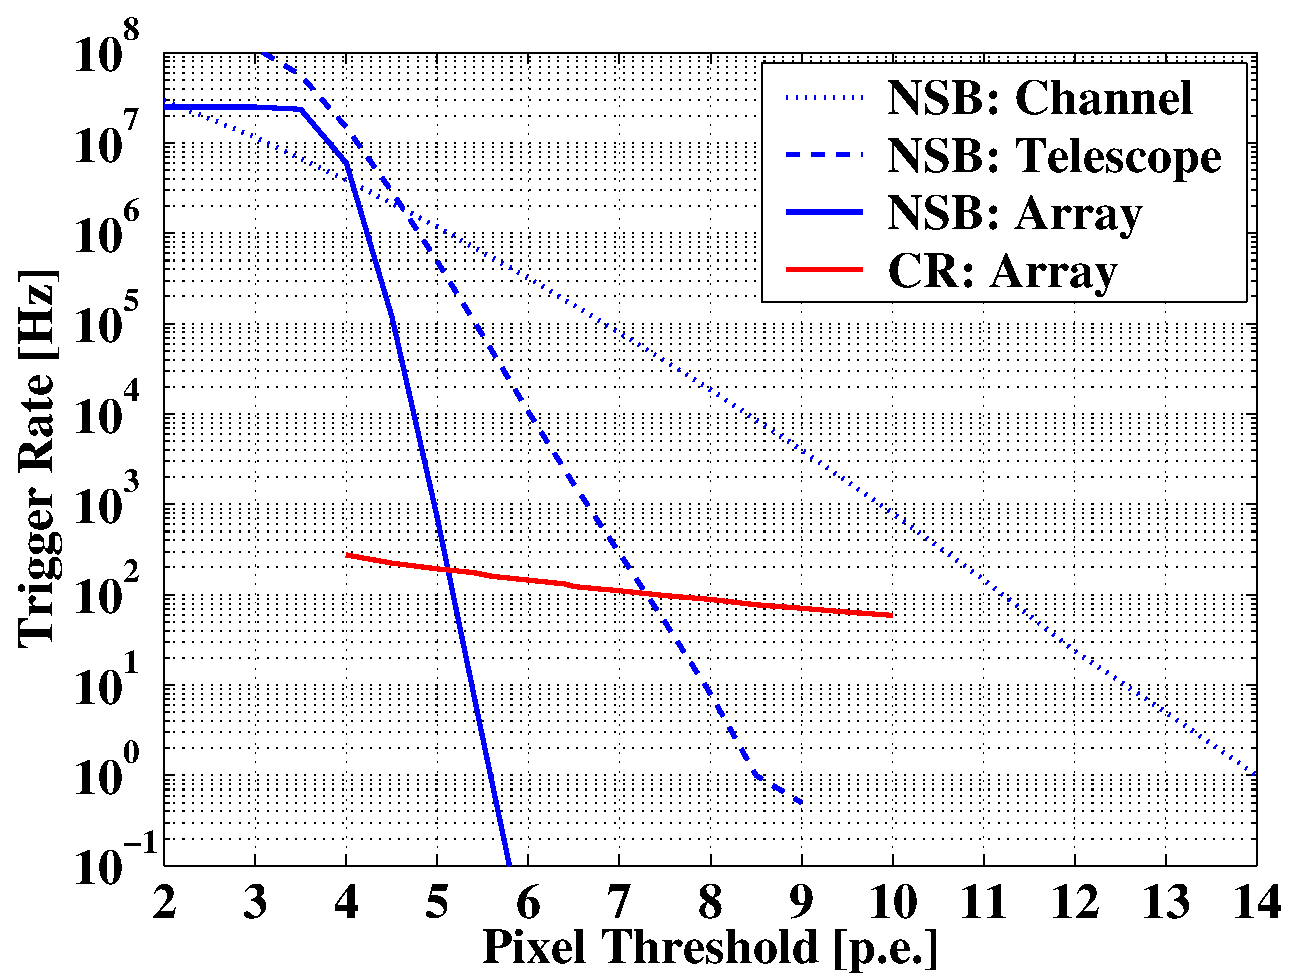
\includegraphics{plots/chap-veritas/TriggerRateColor.pdf}}}
\hspace*{\fill}
\end{minipage}
\caption{\label{FIG::VERITAS::NSB} Triggering rate for L1 (Channel), 
L2 (Telescope) and L3 (Array) vs. pixel trigger threshold (in photo-electrons).
The rate of background cosmic-rays is also shown.}
\end{figure}

A threshold of 5.6\,p.e.\ was chosen as appropriate for 3/4;12m,
corresponding to a trigger rate of $\sim$1\,Hz due to background
light. The array is designed to operate at rates up to 1\,kHz,
corresponding to a threshold of $\sim$5.0\,p.e. However, it can be
seen that the array rate increases rapidly as the trigger threshold is
decreased. The threshold of 5.6\,p.e.\ is chosen for stability and in
order that the simulations will remain largely valid in regions of the
sky where the mean background photon rate is slightly higher than
the 0.16\,ns$^{-1}$\,channel$^{-1}$ assumed valid for dark sky.

\subsection{Simulations database}
\label{SEC::VERITAS::V4SIMULATIONS}

Shower simulations, both \Gray and proton induced, were generated
using the KASCADE simulation package \citep{REF::KERTZMAN::1994NIMA}.
Producing simulated images in the focal plane of an instrument is a
three stage process. In the first stage, KASCADE simulates the
evolution of air-showers initiated by a set of mono-energetic
particles (usually, \Grays or protons) which are randomly injected
into the upper-atmosphere within a certain distance from the center of
the instrument (the ``sampling radius'') at a determined zenith angle.
The package records the particle tracks that join the random interaction
sites in the atmosphere. In the second stage of the simulation,
\Cerenkov light is produced along the particle tracks (if
the particle was charged and had energy above the \Cerenkov threshold)
and propagated through the atmosphere to ground level where all the
surviving photons are recorded. The final stage is to process this
photon database through a simulation of the instrument itself,
accounting for randomly distributed mirror mis-alignments, the
reflectivity of aluminum, mirror weathering, characteristics of the
light concentrators and the wavelength dependent efficiency of the
PMTs. This final stage results in a list of photo-electrons for each
channel and the relative times that they were detected.

The \Gray database for the 12\,m VERITAS array consists of 25
mono-energetic bins, distributed evenly in log(energy) between 10\,GeV
and 10\,TeV with eight bins per decade in energy. The number of events
simulated at each energy decreases with energy reflecting the fact
that many more events are needed at low energies to obtain good
statistics since the triggering efficiency is much lower and hence
most events are not seen by the array. This will be shown in
section~\ref{SEC::VERITAS::V4GAMMARATE}. Conversely, the sampling
radius is increased with energy as large, energetic events are visible
further from the array, the lateral spread of particles in an
energetic air-shower being larger. The sampling radius must be chosen
large enough that a significant fraction of events fail the selection
criteria, in this work the sampling radius was chosen so that a maximum 
of $\sim$85\% of events passed the selection criteria. If this 
requirement failed at any energy the sampling radius was increased. 
All energy bins are produced at a zenith angle of $z=20^\circ$, which 
is considered to be representative of typical observing conditions. 
Table~\ref{TABLE::VERITAS::V4GAMMASIMS} lists the details of four 
representative energy bins.

\begin{table}[ht]
\caption{\label{TABLE::VERITAS::V4GAMMASIMS} Details of the \Gray simulation
database.}
\centerline{\begin{tabular}{lll}\hline
Energy [TeV] & Sampling Radius [m] & Number of Events \\\hline
0.01 & 157.164 & 1197031 \\
0.1  & 209.551 &  146334 \\
1.0  & 304.897 &   14091 \\
10.0 & 376.145 &    1323 \\\hline
\end{tabular}}
\end{table}

The proton-induced database was produced in a similar manner, although
there is an important difference from the \Gray database. The proton
database has four energy bins per decade of energy and each energy bin
consists of 36 sub-bins. This is done to account for the fact that the
cosmic-ray background events are distributed isotropically. For a
\Gray point-source with the telescope pointing directly at the source,
all primaries propagate parallel to the optical-axis of the array. 
This is not true for proton events, so sub-bins are produced with
events originating with angle $\theta$ to the optical axis of the
array. These 36 sub-bins are distributed evenly in $\theta^2$ with
$0^\circ<\theta<6^\circ$. For each of the sub-bins, events are injected
into the atmosphere within a sampling radius, in a similar manner to
the \Gray database.

\subsection{Gamma-ray trigger rate}
\label{SEC::VERITAS::V4GAMMARATE}

To extrapolate from the original work with 10\,m telescopes, the
trigger criteria were applied to the two original configurations
(seven and three telescopes) and to the four telescope array, but with
12\,m aperture instruments: 3/7;12m, 3/3;12m and 3/4;12m. Hence, the
efficiency of each configuration was evaluated over the range of
energies under consideration. In this work, each event was required to
pass the L1, L2 and L3 trigger requirements and was subjected to an
additional requirement aimed at ensuring there is sufficient light in
the image to process it further. To meet this requirement, the events
were conditioned, as described in
section~\ref{SEC::ANALYSIS::CONDITIONING}, and the conditioned images
were required to have at least 25\,p.e. in each of the triggering
telescopes.

Multiplying the area over which the events were sampled,
A$_\mathrm{samp}$\,=\,$\pi$r$_\mathrm{samp}^2$, by the fraction of
events passing the criteria above, leads to an important
characteristic of the array configuration, the \textit{effective
collection area} for {\Grayc}s. This characteristic is essentially the
detector area that an equivalent, 100\% efficient, ``space-based''
instrument would require to detect the same flux of \Grays
directly. Figure~\ref{FIG::VERITAS::EFFAREA} shows how the effective
area depends on energy for the three configurations. After the
hadronic rejection cuts are applied the effective area is suppressed
by a factor of approx. 30\%--70\%, as shown in
section~\ref{SEC::VERITAS::V4CUTS}.

\begin{figure}[p]
\begin{minipage}{\textwidth}
\hspace*{\fill}
\resizebox{0.7\textwidth}{!}{\rotatebox{270}{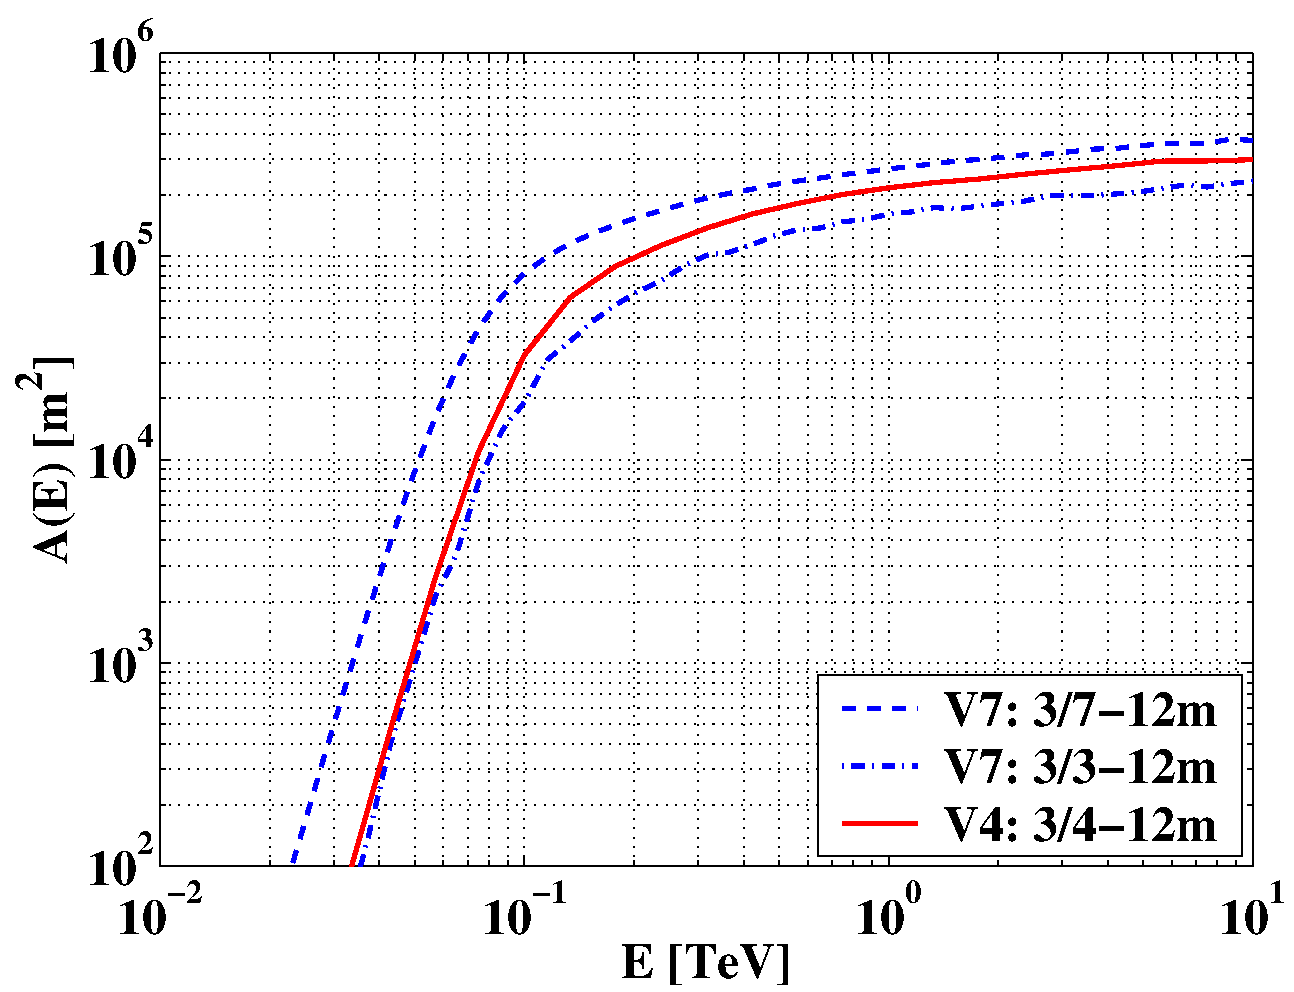
\includegraphics{plots/chap-veritas/InterpolationCollectionAreaColor.pdf}}}
\hspace*{\fill}
\end{minipage}
\caption{\label{FIG::VERITAS::EFFAREA} Effective areas for various array
configurations.}
\end{figure}

Another characteristic of interest is the energy at which most \Grays
are detected, for a given \Gray source spectrum, typically the Crab
Nebula spectrum \citep{REF::HILLAS::1998}, approximated here by a
power-law over the energy range of 10\,GeV to 100\,TeV:
\[\mathrm{\frac{dF}{dE}=3.2\times10^{-7}\left(\frac{E}{TeV}\right)^{-2.5}\,
m^{-2}\,s^{-1}\,TeV^{-1}}\] 
The \textit{differential rate}, given by,
\[\mathrm{\frac{dR}{dE}(E) = A(E)\frac{dF}{dE} = 3.2\times10^{-7}\,A(E)\,
\left(\frac{E}{TeV}\right)^{-2.5}\;s^{-1}\,TeV^{-1}}\]
is shown for the 3/4;12m array criterion in
figure~\ref{FIG::VERITAS::DIFFRATE}. The energy at which this curve is
reaches a maximum, often called the peak detection energy, or
E$_\mathrm{peak}$, is 110\,GeV. Integrating the curve gives a total
triggering rate of $\sim45$\,min$^{-1}$ from the Crab
Nebula. Approximately 10\% of the detected events have energies less
than 100\,GeV, and 10\% have energy greater than 1\,TeV. These results
are summarized in table~\ref{TABLE::VERITAS::DIFFRATE}.

\begin{figure}[p]
\begin{minipage}{\textwidth}
\hspace*{\fill}
\resizebox{0.7\textwidth}{!}{\rotatebox{270}{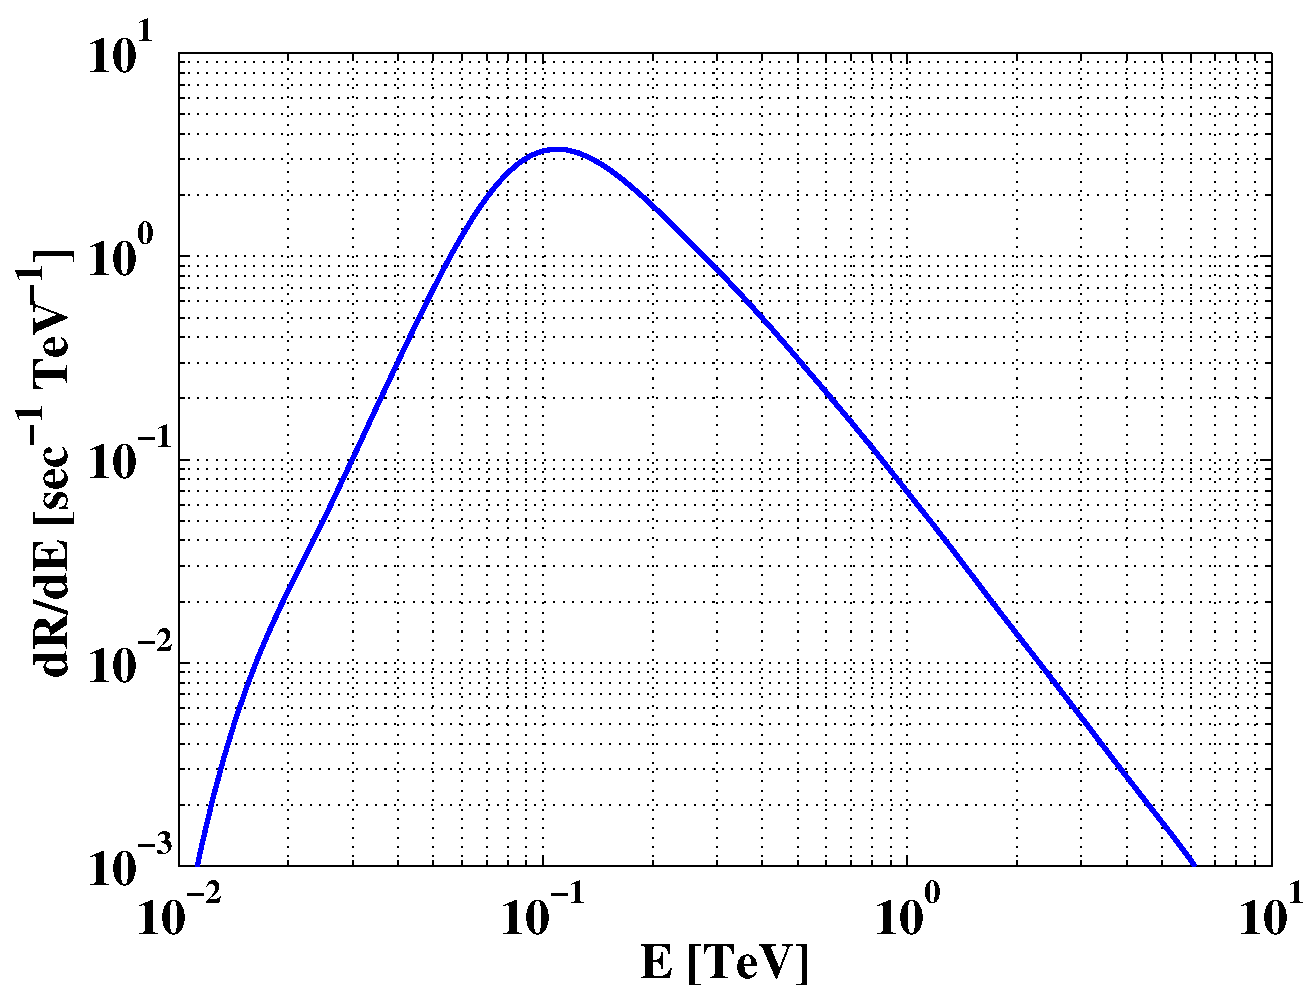
\includegraphics{plots/chap-veritas/DifferentialRateColor.pdf}}}
\hspace*{\fill}
\end{minipage}
\caption{\label{FIG::VERITAS::DIFFRATE} Differential rate for a Crab Nebula 
like source. The energy at which the detected rate is maximal is, 
E$_\mathrm{peak}$=110\,GeV.}
\end{figure}

\begin{table}[t]
\caption{\label{TABLE::VERITAS::DIFFRATE} Summary of collection area and 
integral rate from Crab Nebula.}
\centerline{\begin{tabular}{lll}\hline
& Collection area & \Gray rate \\
\raisebox{1.5ex}[0ex]{Energy} & [m$^2$] & $>$ E [min$^{-1}$] \\\hline
30\,GeV  & 2.0$\times$10$^2$ & 45 \\
100\,GeV & 3.3$\times$10$^4$ & 40 \\
300\,GeV & 2.2$\times$10$^5$ & 15 \\
1\,TeV   & 3.0$\times$10$^5$ &  4 \\\hline
\end{tabular}}
\end{table}

\subsection{Effect of shape- and aperture-cuts}
\label{SEC::VERITAS::V4CUTS}

The effects of the shape- and aperture-cuts are interpolated from the
full analysis of the 3/3;10m and 3/7;10m configurations. For each of
these two cases a function A(E,~$\theta_\mathrm{cut}$), corresponding
to the effective area of the array at energy E with optimum shape-cut
and aperture-cut given by $\theta_\mathrm{cut}$, is shown in
figure~\ref{FIG::VERITAS::CUTS}. This surface was derived by
polynomial interpolation from four curves available from the full
analysis. These are A(E,~$\pi$), the effective area with no
aperture-cuts applied, i.e.\ trigger and optimized shape-cut
only. This curve is shown as the top-left plot of
figure~\ref{FIG::VERITAS::CUTS}. The remaining three curves used to
interpolate the surface were A(100\,GeV,~$\theta_\mathrm{cut}$),
A(1\,TeV,~$\theta_\mathrm{cut}$) and
A(10\,TeV,~$\theta_\mathrm{cut}$), the effective area for three energy
bins with trigger, optimized shape-cut and an aperture-cut of varying
degrees applied. These three curves are shown for both array
configurations in the bottom-left plot in
figure~\ref{FIG::VERITAS::CUTS}.

\begin{figure}[t]
\begin{minipage}{\textwidth}
\hspace*{\fill}
\begin{minipage}[t]{0.3\textwidth}
\resizebox{\textwidth}{!}{\rotatebox{270}{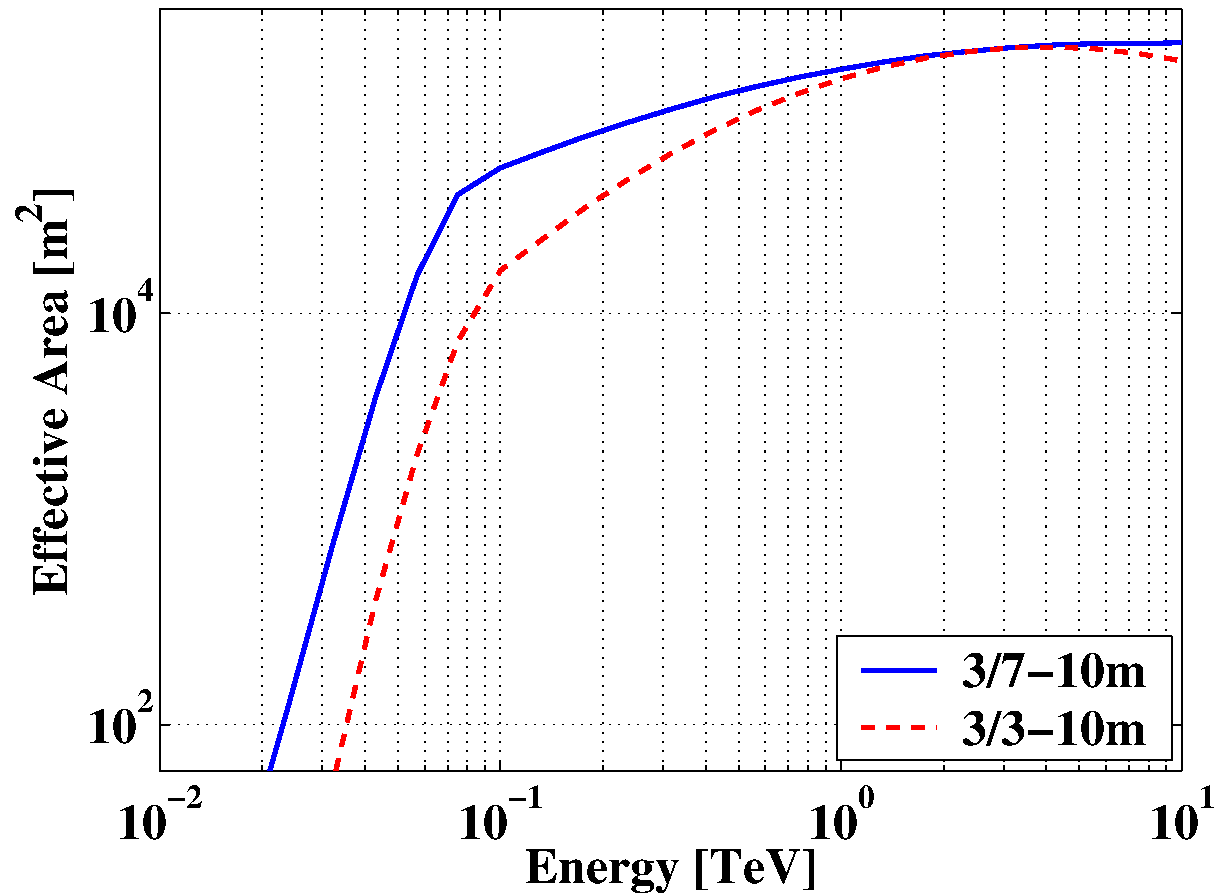
\includegraphics{plots/chap-veritas/V7CollectionAreaColor.pdf}}}
\resizebox{\textwidth}{!}{\rotatebox{270}{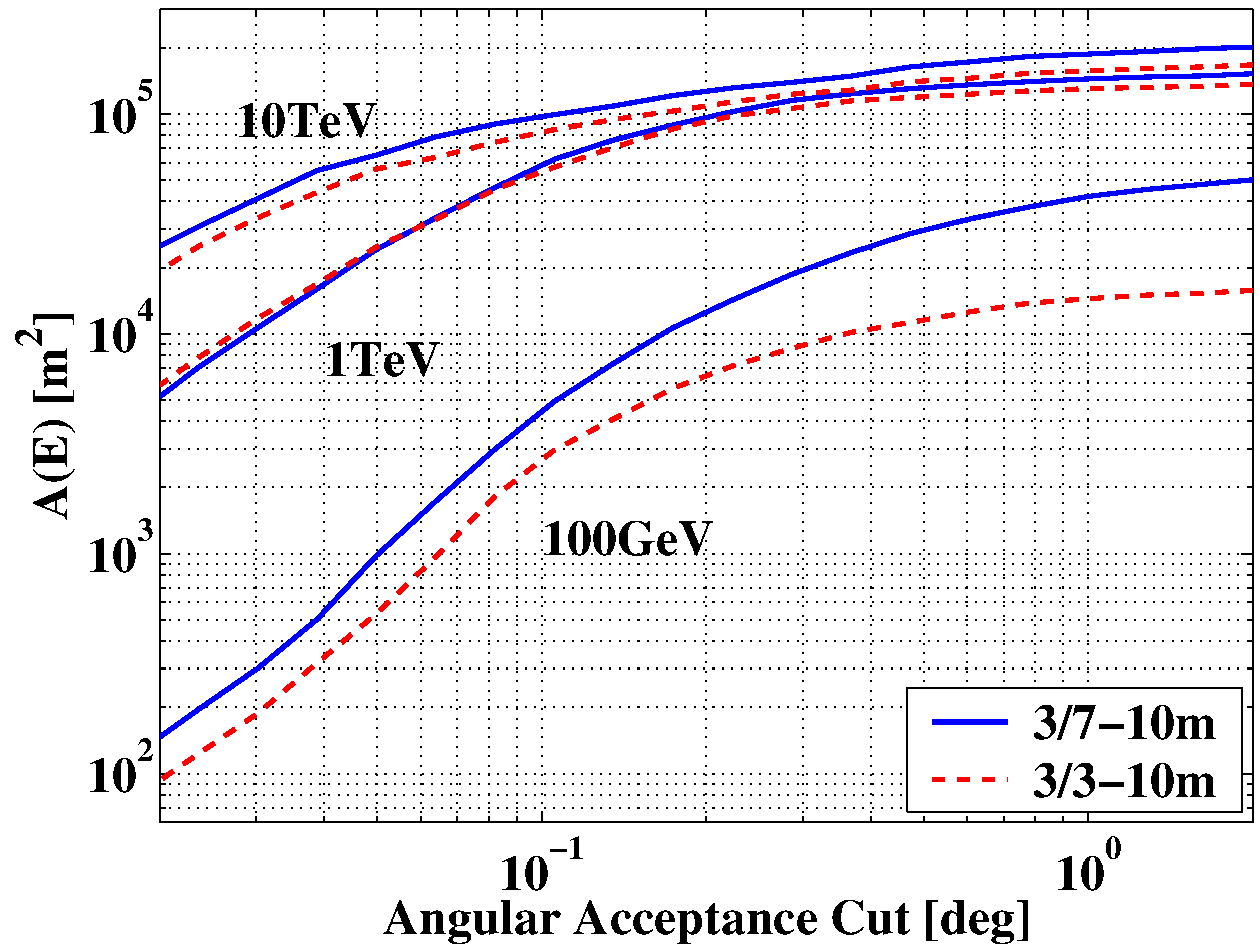
\includegraphics{plots/chap-veritas/V7ApertureCollectionAreaColor.pdf}}}
\end{minipage}
\resizebox{0.68\textwidth}{!}{\rotatebox{270}{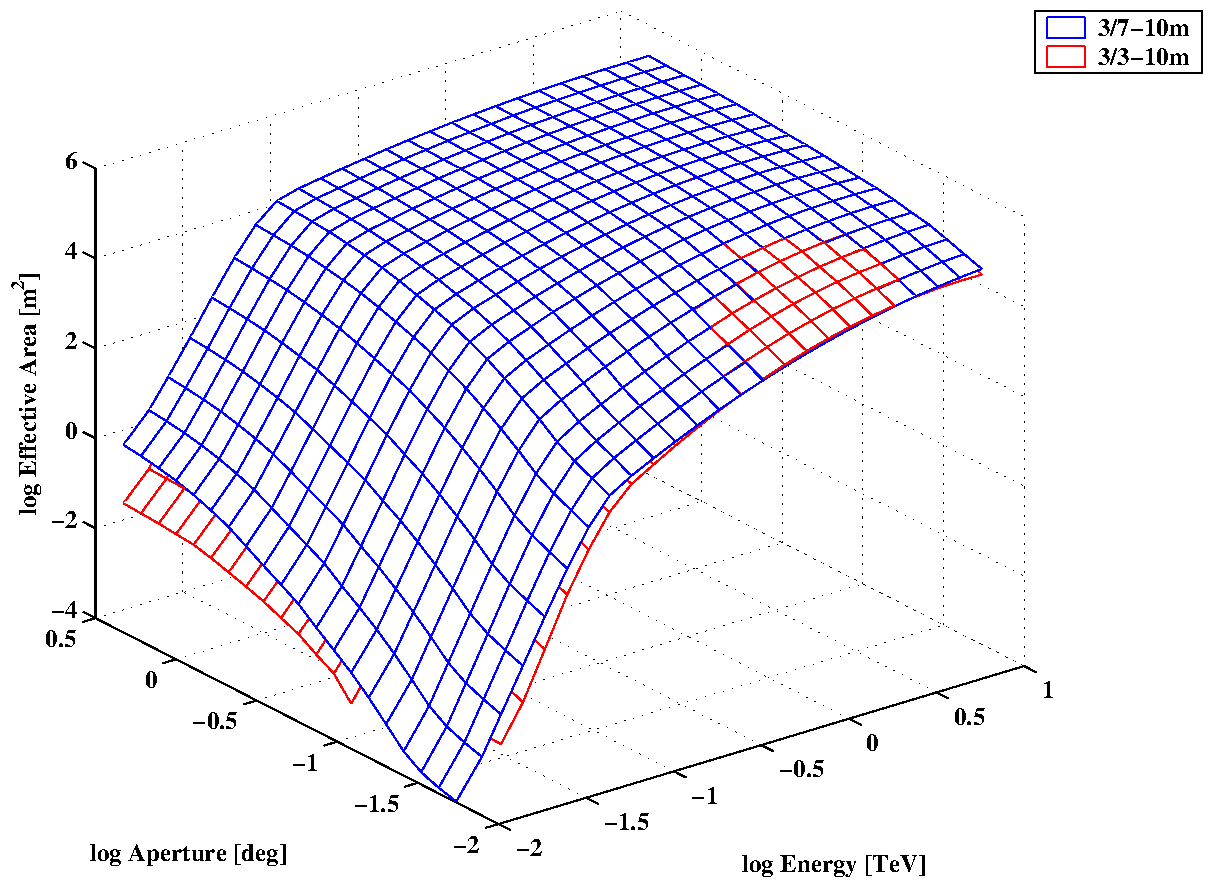
\includegraphics{plots/chap-veritas/V7MeshCollectionAreaColor.pdf}}}
\hspace*{\fill}
\end{minipage}
\caption{\label{FIG::VERITAS::CUTS} (Left-Top) Effective area with shape cut 
applied. (Left-Bottom) Effective area with shape and aperture-cuts applied 
vs. aperture-cut for three energies. (Right) A(E, $\theta_\mathrm{cut}$), 
effective area surface with shape and aperture-cuts applied.}
\end{figure}

The A(E,~$\theta_\mathrm{cut}$) surface applicable to the 3/4;12m
configuration is interpolated from the 3/3;10m and 3/7;10m by scaling
using the trigger effective area curves on
figure~\ref{FIG::VERITAS::EFFAREA} and the equivalent curves for the
10\,m case. From here on the effective area curve for the 10\,m case with
only the trigger cut applied is referred to as $\mathrm{A^{TR}_{X;10m}(E)}$
(with X=3/3, 3/7 or 3/7), with a similar expression for the 12\,m
case. The effective area surface with trigger, shape-cut and
aperture-cuts applied is similarly referred to as
$\mathrm{A^{SA}_{X;10m}(E,~\theta_\mathrm{cut})}$.

Defining the ratio of the trigger-only effective areas in the 12\,m and
10\,m cases as $R\mathrm{_X(E)}$, i.e.\
\[R\mathrm{_X(E) = \frac{A^{TR}_{X;12m}}{A^{TR}_{X;10M}}}\]
and $x(\mathrm{E})$ as the interpolation factor between the 3/4 trigger-only
curve and the 3/3 and 3/7 trigger-only curve in log space,
\[x(\mathrm{E}) = \mathrm{\frac{\log A^{TR}_{3/4;12m}(E) - \log A^{TR}_{3/3;12m}(E)}
{\log A^{TR}_{3/7;12m}(E) - \log A^{TR}_{3/3;12m}(E)}}\]
Then the 3/4;12m effective area with trigger, shape-cut and
aperture-cut applied is the interpolation between the 3/3;10m and 3/7;10m
cases,
\begin{eqnarray*}
\mathrm{\log A^{SA}_{3/4;12m}(E,\;\theta_{cut})} & = &
x(\mathrm{E})\,\log \left\{R_{3/3}(\mathrm{E})\,\mathrm{A^{SA}_{3/3;10m}(E,\;\theta_{cut})}\right\}\,+\\
& & (1-x(\mathrm{E}))\,\log \left\{R_{3/7}(\mathrm{E})\,\mathrm{A^{SA}_{3/7;10m}(E,\;\theta_{cut})}\right\}
\end{eqnarray*}

\subsection{Angular resolution}
\label{SEC::VERITAS::V4ANGRESOLUTION}

The optimum aperture cut, $\theta_\mathrm{cut}(E)$, is calculated by
maximizing the detected \Gray significance (signal-to-noise ratio) at
each energy.  Figure~\ref{FIG::VERITAS::ANGULAR} (left) shows a plot
of the probability for event reconstruction, based on collection area
A(E,~$\theta_\mathrm{cut}$), for three different energies. This
corresponds to the probability of reconstructing a \Gray within
$\theta_\mathrm{cut}$ of its arrival direction, denoted
P$_\gamma$($<\theta_\mathrm{cut}$). The probability of reconstructing
the event within $\pi$ is unity, dropping off as tighter cuts are
made. It can be seen from the probability curves that high energy
events are reconstructed more accurately than low-energy events. A cut
of 1 arc minute excludes 90\% of 10\,TeV events, 97\% of 1\,TeV events
and $>$99\% of 100\,GeV events. Interestingly, there is a range of
aperture cut for which mid-energy \Grays have higher probability to
pass than the highest energy events. This is likely a result of
``clipping'' of the shower image in the camera, an effect of the
higher energy showers developing deeper into the atmosphere and being
longer in angular extent than the low energy showers.

\begin{figure}[t]
\resizebox{0.49\textwidth}{!}{\rotatebox{270}{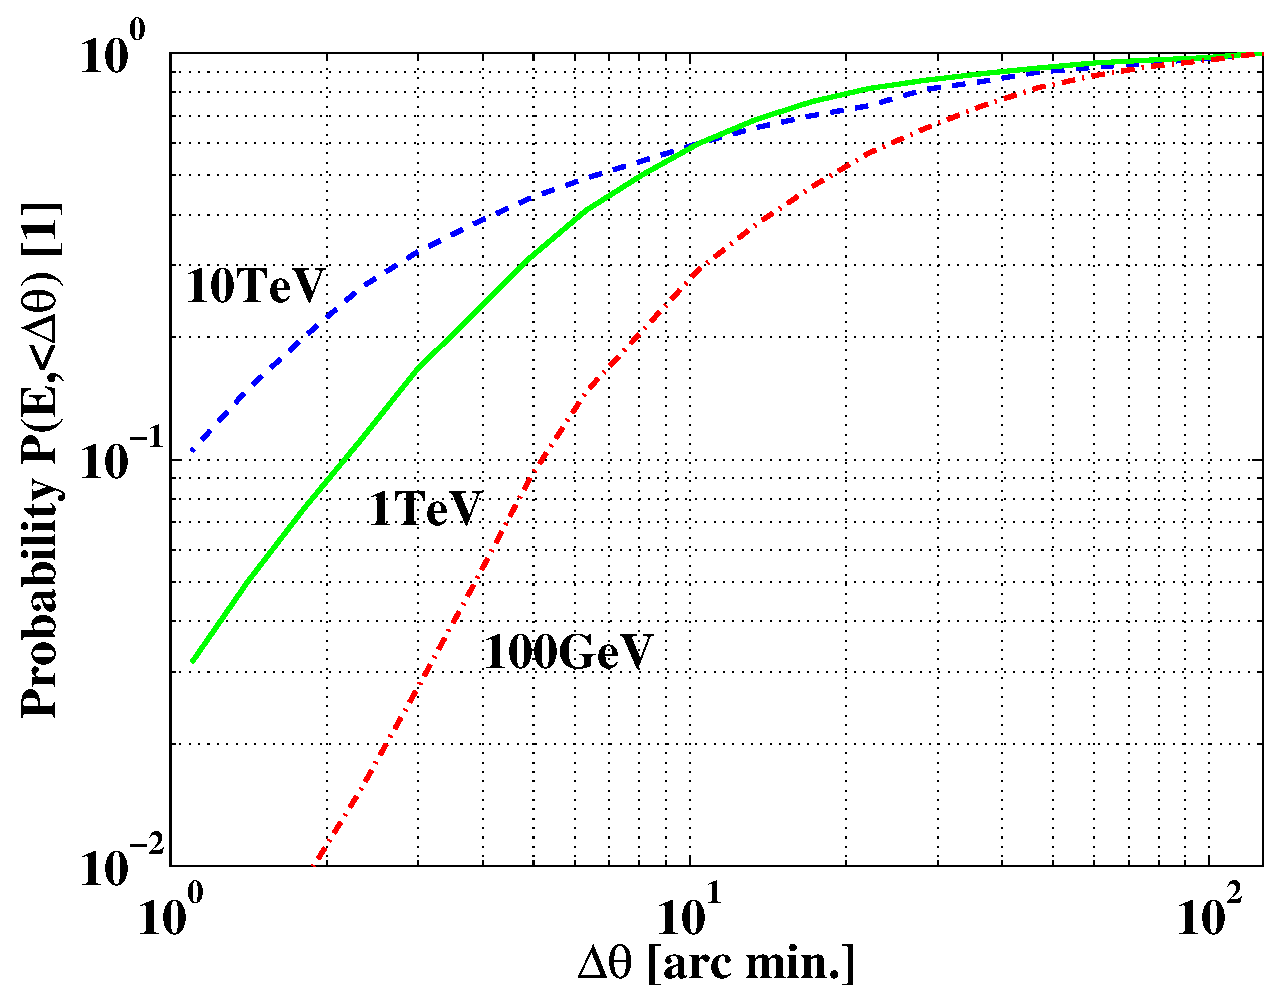
\includegraphics{plots/chap-veritas/AngularErrorColor.pdf}}}
\resizebox{0.49\textwidth}{!}{\rotatebox{270}{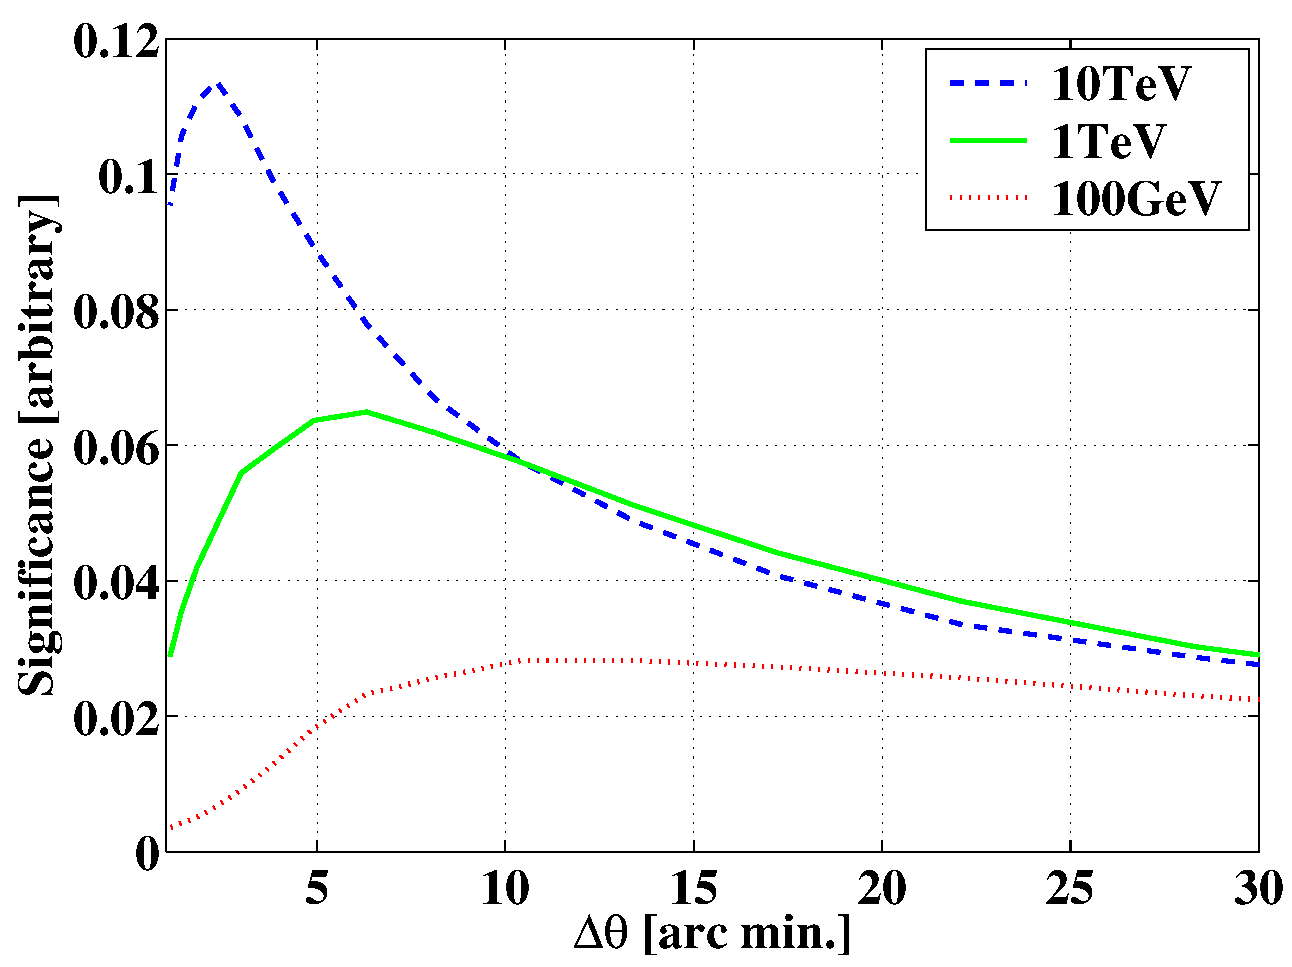
\includegraphics{plots/chap-veritas/AngularAcceptanceColor.pdf}}}
\caption{\label{FIG::VERITAS::ANGULAR} (Left) P(E,$<\theta_\mathrm{cut}$), 
probability that a \Gray event with certain energy will be
reconstructed closer than $\theta_\mathrm{cut}$ to the true
origin. (Right) Significance of \Gray events over isotropic background
events.}
\end{figure}

The number of isotropic background cosmic-ray events passing an
angular cut is,
P$_\mathrm{p}$($<\theta_\mathrm{cut}$)$\propto\theta^2_\mathrm{cut}$,
to first order in $\theta_\mathrm{cut}$. The detection significance ratio is
therefore,
\[\mathrm{\sigma(\theta_{cut})\propto
\frac{P_\gamma(<\theta_{cut})}{\sqrt{P_p(<\theta_{cut})}}\propto
\frac{P_\gamma(<\theta_{cut})}{\theta_\mathrm{cut}}}\]
Figure~\ref{FIG::VERITAS::ANGULAR} (right) shows the significance at
three energies. Maximizing the detection significance at every energy
gives the optimized values for the aperture cut,
$\theta^*_\mathrm{cut}(E)$. To evaluate the angular resolution of the
instrument, a fit is made to
dP$_\gamma$($<\theta_\mathrm{cut}$)/d$\theta_\mathrm{cut}$ in the
region of $\theta_\mathrm{cut}(E)<\theta^*_\mathrm{cut}(E)$ with the
assumption that the reconstructed events are distributed as a
two-dimensional Gaussian. The half-width of the fitted Gaussian is
defined as the angular-resolution of the
instrument. Table~\ref{TABLE::VERITAS::ANGULAR} gives the optimized
aperture-cut and the angular resolution of three \Gray energies. In
section~\ref{SEC::VERITAS::V4SENSITIVITY} a more useful method of
calculating the optimum aperture-cut by directly maximizing the
sensitivity of the instrument to \Grays is described. It is
%essentially analogous 
similar to the method shown here, the main difference
being a more accurate treatment of the background.

\begin{table}[t!]
\caption{\label{TABLE::VERITAS::ANGULAR} Summary of angular resolution
and optimized aperture cuts for VERITAS-4.}
\centerline{\begin{tabular}{lllll}\hline
& \multicolumn{2}{c}{Optimized aperture cut} 
& \multicolumn{2}{c}{Angular resolution} \\
\raisebox{1.5ex}[0pt]{Energy} & [arc. min] 
& [degrees]& [arc. min] & [degrees]\\\hline
10\,TeV  &  2' & 0.03$^\circ$ & 1.6' & 0.03$^\circ$ \\
1\,TeV   &  6' & 0.10$^\circ$ & 4.3' & 0.07$^\circ$ \\
100\,GeV & 11' & 0.18$^\circ$ & 7.5' & 0.13$^\circ$ \\\hline
\end{tabular}}
\end{table}

\subsection{Cosmic-ray events}
\label{SEC::VERITAS::V4CR}

%\enlargethispage{12pt}
As noted in section~\ref{SEC::VERITAS::V7REJECTION} the
energy-estimator function is chosen and optimized with \Gray images,
with the requirement that
\mbox{E$_\mathrm{est}\approx$\,E$_\gamma$}. This will not, in general,
be the case for hadronic showers whose images are inherently different
from \Gray images of the same energy. In a full simulation of the
array performance where the reconstruction technique is applied to
hadronically-induced events, the energy-estimator will assign a
``\Grayc-energy estimate'', E$_{est}$ to each hadronic event of energy
E$_\mathrm{p}$. These events will then naturally be counted toward the
background in the energy bin containing E$_{est}$, when the instrument
sensitivity is calculated.

For this work, since the full reconstruction is not applied to the
data, a different approach to finding the equivalent \Grayc-energy is
adopted. An assumption is made that, for those hadronic showers that
result in \Grayc-like images, the energy estimate is, to first order,
a function of the amount of light collected relative to the amount of
light an equivalent \Gray event would produce. It is found that the
following relationship holds, except possibly at the lowest energies,
\[ \mathrm{\frac{E_{est}}{TeV} \approx 0.4 \frac{E_p}{TeV}^{0.88}} \]
Using this expression the proton spectrum of 
\[\mathrm{\frac{dF}{dE_p}=1.1\times10^{-5}
\frac{E_p}{TeV}^{-2.75}\,m^{-2}\,s^{-1}\,TeV^{-1}\,sr^{-1}}\] 
can be converted into a spectrum in equivalent \Gray energy,
E$_\gamma$.  By folding this spectrum with the collecting area for
protons, also expressed in equivalent \Gray energy the differential
rate of detected cosmic-ray events is calculated,
figure~\ref{FIG::VERITAS::CR}.

\begin{figure}[ht]
\resizebox{0.49\textwidth}{!}{\rotatebox{270}{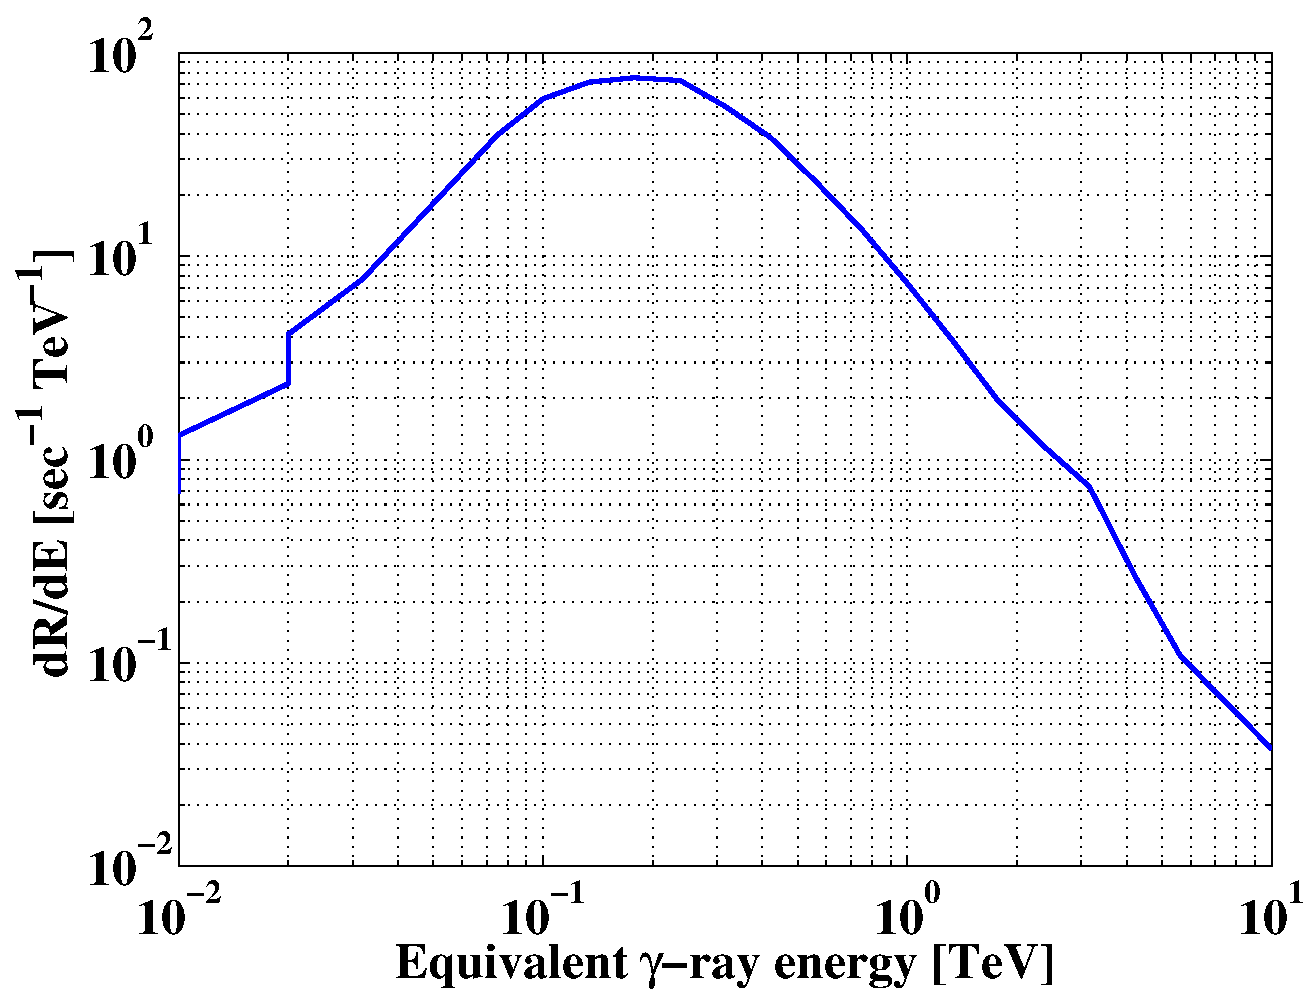
\includegraphics{plots/chap-veritas/ProtonDifferentialRateColor.pdf}}}%
\resizebox{0.49\textwidth}{!}{\rotatebox{270}{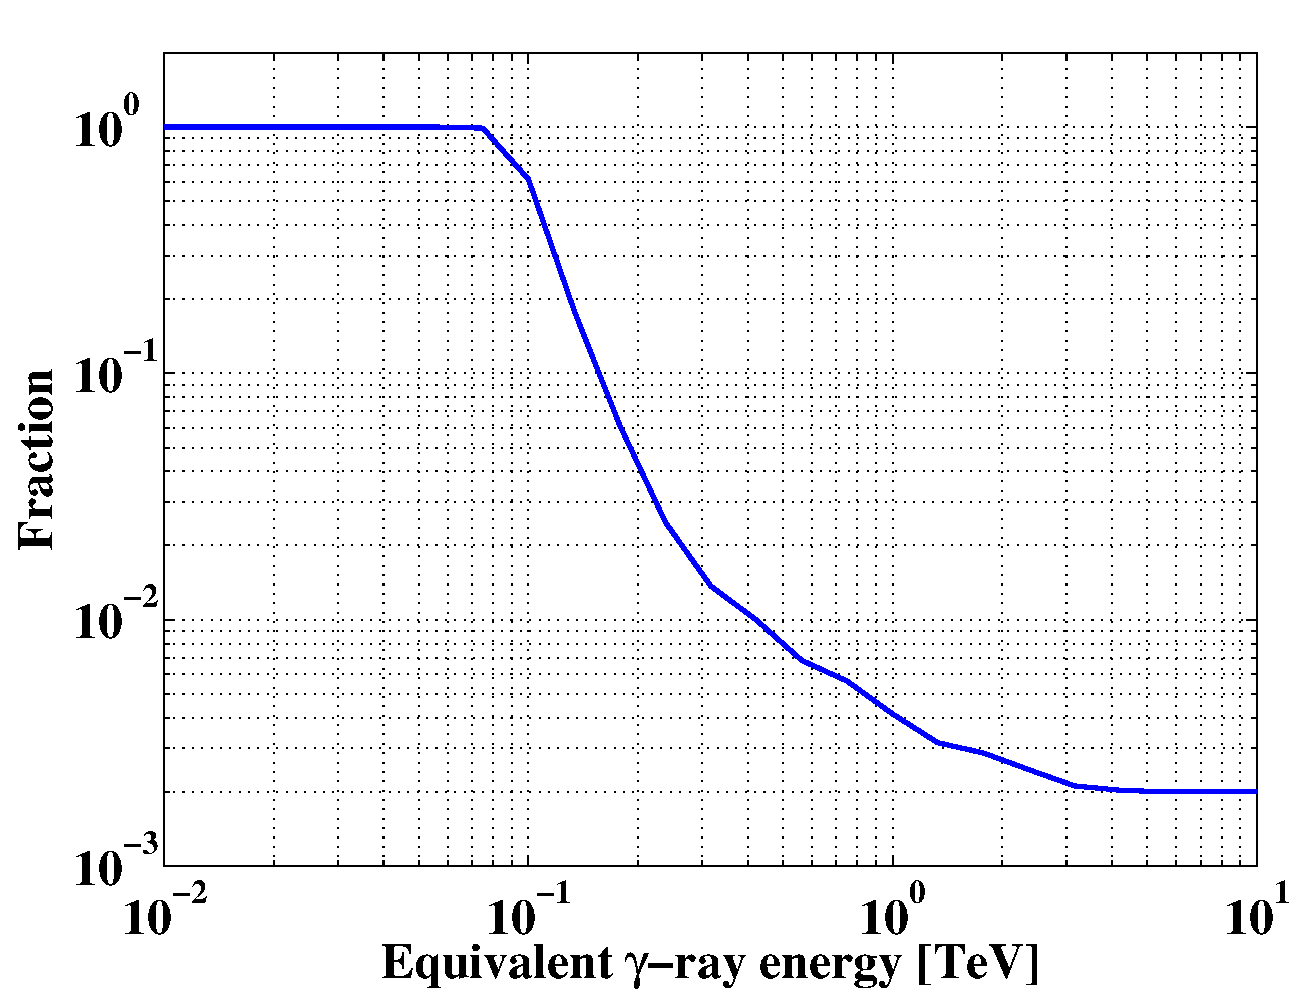
\includegraphics{plots/chap-veritas/ProtonSuppressionFactorColorBB.pdf}}}
\caption{\label{FIG::VERITAS::CR} (Left) Differential rate of background 
cosmic-ray events, expressed in equivalent \Gray energy. (Right)
Fraction of background events passing shape-cuts.}
\end{figure}

%\enlargethispage{12pt}
The fraction of background events passing the ``shape-cut'' was
determined during the comprehensive evaluation of VERITAS
characteristics and is plotted in figure~\ref{FIG::VERITAS::CR}
(right) for completeness. It is assumed that this curve is applicable
to the updated VERITAS configuration.  This assumption, although not
completely accurate, is reasonable, since the shape cut on $D$ (as
explained in section~\ref{SEC::VERITAS::V7REJECTION}) does not depend
strongly on mirror size. The absolute value of $D$ for any event has a
dependence on mirror diameter from its definition as the RMS distance
from the back-traced rays to the image axis, with the back-traced rays
being reflected off the entire mirror area. The average value of $D$,
for events of any given energy, will increase from the 10\,m to the
12\,m case. The dispersion in $D$ will also increase for events of a
given \Gray energy, decreasing the efficiency of any cut on
$D$. However this will be compensated for, to some extent, by an
increase in the amount of light collected for each event, giving more
collected photons and a better estimate of $D$.

\subsection{Sensitivity}
\label{SEC::VERITAS::V4SENSITIVITY}

The sensitivity of an atmospheric \Cerenkov imaging telescope to a
\Gray source is usually expressed as the minimum observable flux the
source must have to be detected with a certain significance in a
certain exposure time. A minimum flux sensitivity is calculated for a
range of energy bins, separated equally in log(energy) with four bins
per decade. This configuration of energy bins is the same as that used
when attempting to reconstruct the energy spectrum of a detected
source.

Given an exposure of duration $\Delta T$ and \Gray detection rate of
$R_\gamma$ with background event rate of $R_B$, the number of counts
collected while observing the source is $N_{ON}=(R_\gamma+R_B) T$. The
number of events collected while taking a control observation, in the
absence of the source is $N_{OFF}=R_B T$. The significance of the
detection is therefore
\[ \sigma=\frac{N_{ON}-N_{OFF}}{\sqrt{N_{ON}+N_{OFF}}}=
\frac{R_\gamma T}{\sqrt{(R_\gamma+2R_B) T}} \]

Given any required significance, this expression can be solved for
$R_\gamma$ (the positive root) giving,
\[ R_\gamma = 
\sigma^2\left\{\frac{1+\sqrt{1+8R_B T/\sigma^2}}{2 T}\right\} \]

The background has two significant components; cosmic-rays and
cosmic-electrons. The cosmic-ray flux is calculated by integrating the
differential proton rate, figure~\ref{FIG::VERITAS::CR} (left),
multiplied by the fraction of cosmic-ray events passing the shape
cuts, figure~\ref{FIG::VERITAS::CR} (right). The rate of detected
electrons is given by integrating the differential flux of the
cosmic-electrons,
\[\mathrm{\frac{dF}{dE_{e^{\pm}}}=9.5\times10^{-9}\frac{E_{e^{\pm}}}{TeV}^{-3.26}\,m^{-2}\,s^{-1}\,TeV^{-1}\,sr^{-1}}\] 
multiplied by the \Gray collecting area and by the angular-extent of
the aperture-cut, $\pi\theta_\mathrm{cut}^2$.

The minimum observable rate in an energy bin centered at
$\mathrm{E_c}$, given by $\mathrm{R_\gamma(E_c)}$ can then be
converted into a minimum observable flux,
$\mathrm{F_\gamma(10^{-1/8}E_c\rightarrow 10^{+1/8}E_c)}$, by dividing
by the \Gray collection area. The flux is usually expressed
differentially in flux units as $\mathrm{E\,dF/dE}$ or in power units
as $\mathrm{E^2\,dF/dE}$ by assuming a power-law spectrum
$\mathrm{dF/dE=F^*E^{-(\Gamma+1)}}$,
\[\mathrm{R_\gamma(E_c)} = 
\int_{10^{-1/8}\mathrm{E_c}}^{10^{+1/8}\mathrm{E_c}}
\mathrm{A}(E')\mathrm{F}^*E'^{-(\Gamma+1)}dE' \approx
\mathrm{F^*(E_c)A(E_c)E_c^{-\Gamma}
\left(\frac{10^{+1/8\Gamma}-10^{-1/8\Gamma}}{\Gamma}\right) }\] 
assuming four bins per decade of energy, whose edges ($10^{-1/8}E_c$
and $10^{+1/8}E_c$) are equally spaced around $\mathrm{E_c}$ in log
space. It is also assumed that the collecting area $\mathrm{A}(E')$
changes slowly within each bin and can be replaced in the integration
with its value at the center of the bin. The expression in the
parentheses, a product of the binning and the assumed power-law index,
can be written as the constant $\mathrm{B}$. Hence,
\[\mathrm{E\,\frac{dF}{dE}=F^*E^{-\Gamma}\approx 
\frac{R_\gamma(E)}{B \times A(E)}}\]

In the original VERITAS-7 work, the sensitivity was derived as a
function of energy, shape-cut and aperture-cut, i.e.\ as
$\mathrm{E\,\frac{dF}{dE}}(\mathrm{E},~D_{\mathrm{cut}},
~\theta_{\mathrm{cut}})$. It was by maximizing this function for every
energy bin that the optimum values of $D_{\mathrm{cut}}(\mathrm{E})$
and $\theta_{\mathrm{cut}}(\mathrm{E})$ were found. For this analysis,
the value of the optimum shape-cut was taken implicitly from the
previous analysis.  The optimum aperture-cut was calculated by
maximizing the sensitivity, taken as a function of energy and
aperture-cut, $\mathrm{E\,\frac{dF}{dE}}(\;\mathrm{E},
~\theta_{\mathrm{cut}}\;|\;D_{\mathrm{cut}}(\mathrm{E})\;)$, with the
shape-cut fixed as described above.

Figure~\ref{FIG::VERITAS::SENSITIVITY} shows the sensitivity of the
VERITAS-4 array to \Gray sources. In each region of this plot a
different background dominates. For the case of 50\,hrs exposure, in
the region E$>$2\,TeV the limitation is \Gray statistics, a minimum of
25 counts are needed for a $5\sigma$ detection. At $\sim$1\,TeV the
most prominent background is cosmic-ray interactions producing only
$\pi^0$ particles which decay and initiate purely electromagnetic
showers. These events cannot be differentiated from \Gray events. At
200\,GeV$<$E$<\sim$1\,TeV cosmic-ray and cosmic-electron initiated
events dominate approximately equally. At low energies, night sky
noise affects the images of all events strongly degrading the
performance of the \Gray separation.

It can be seen from the diagram that VERITAS will be sensitive to a
source as bright as the Crab Nebula between 30\,GeV and $>$30\,TeV in
50 hours of observations. This will provide a large overlap with
next generation satellite-based instruments which are expected to
operate up to energies of 300\,GeV 
\citep{REF::NASA::2001GLASTPROPOSAL}.

\begin{figure}[t]
\resizebox{\textwidth}{!}{\rotatebox{270}{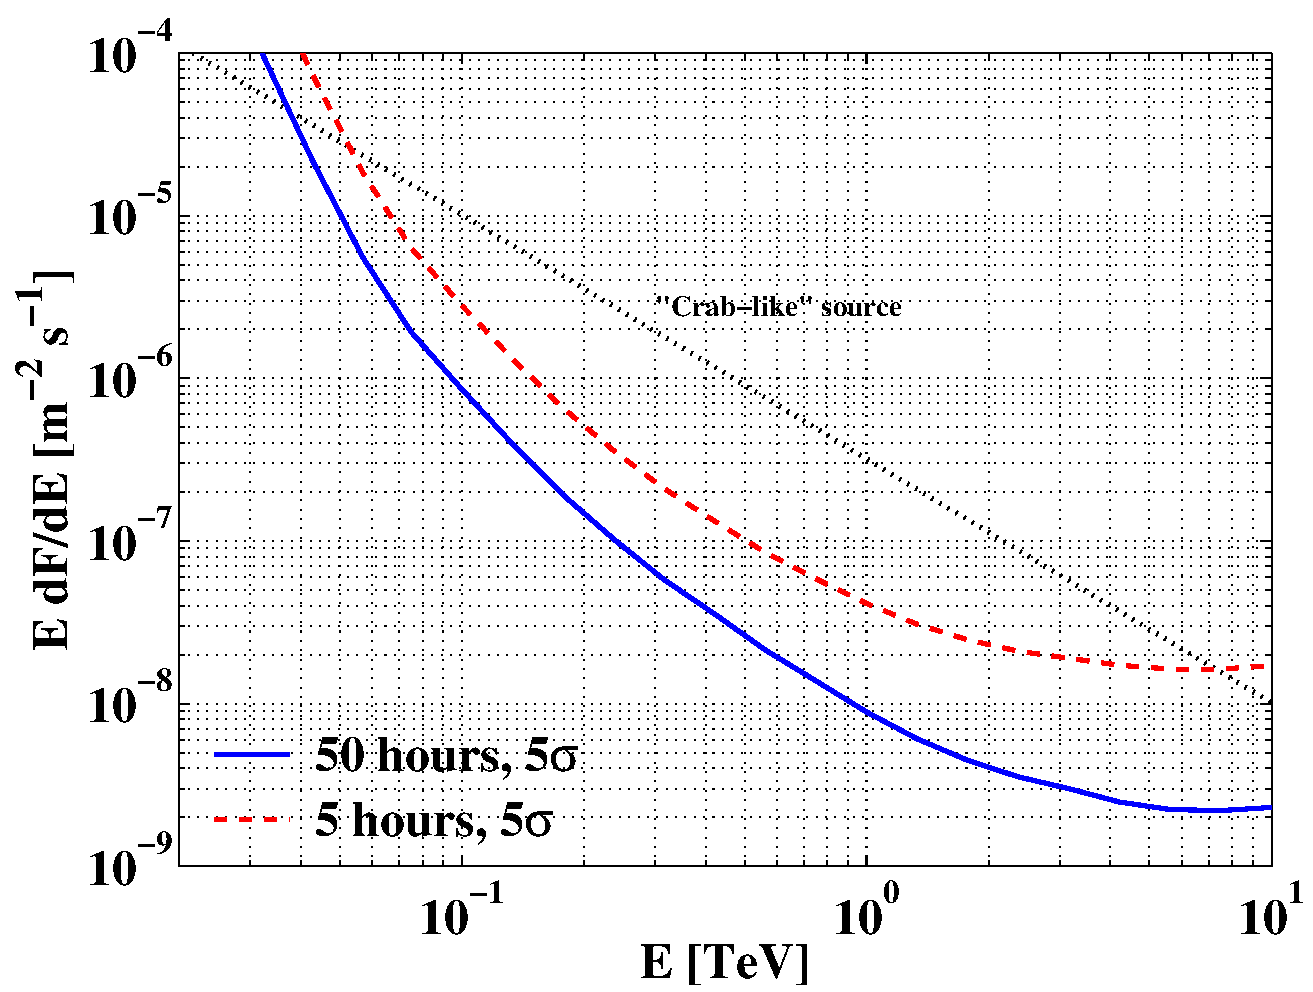
\includegraphics{plots/chap-veritas/Sensitivity50and5Color.pdf}}}
\caption{\label{FIG::VERITAS::SENSITIVITY} Minimum observable \Gray flux
for 50 and 5 hour observations with the VERITAS-4 array given a
required detection significance of 5$\sigma$ in each energy bin. The
sensitivity is quoted for energy bins separated equally in log(energy)
with four bins per decade.}
\end{figure}

\section{Summary of results}
\label{SEC::VERITAS::SUMMARY}

These results were presented to the VERITAS funding agencies to show
the worthiness of a first stage, four telescope instrument. The
configuration, with 12\,m telescopes, performs well in comparison to
the full VERITAS 7$\times$10\,m instrument although there is an
inevitable loss of sensitivity at the lowest energies (below 100\,GeV)
and less flexibility to split the instrument into sub-array
configurations. Partially on the basis of these results, the four
telescope instrument has been funded; a prototype is being built at
the Smithsonian Astrophysical Observatory facility close to the
original Montosa canyon site. Construction of the full instrument will
begin at Horseshoe canyon on Kitt Peak in 2004. This new site, at
higher elevation, will allow the instrument to exceed the
specifications calculated here and summarized in
table~\ref{TABLE::VERITAS::SUMMARY}.

\begin{table}[p]
\caption{\label{TABLE::VERITAS::SUMMARY} Summary of the characteristics of
the VERITAS-4 sub-array.}
\centerline{\begin{tabular}{lll}\hline
Characteristic & E & Value \\ \hline
Peak Energy $^a$ & & 110 GeV \\
Flux sensitivity$^b$ & at 100\,GeV & 3.4$\times$10$^{-11}$cm$^{-2}$s$^{-1}$ \\
 & at 1\,TeV & 6.5$\times$10$^{-13}$cm$^{-2}$s$^{-1}$ \\
 & at 10\,TeV & 2.1$\times$10$^{-13}$cm$^{-2}$s$^{-1}$ \\
Angular resolution$^c$ & 100\,GeV & 7.5 arc min \\
 & 1\,TeV & 4.3 arc min \\
 & 10\,TeV & 1.6 arc min \\
Collection area$^d$ & 100\,GeV & 3.3$\times$10$^8$cm$^2$ \\
 & 1\,TeV & 2.2$\times$10$^9$cm$^2$ \\
 & 10\,TeV & 3.0$\times$10$^9$cm$^2$ \\
Crab Nebula & $>$30\,GeV & 45/minute \\
$\gamma$-ray rates$^e$ & $>$100\,GeV & 40/minute \\
 & $>$300\,GeV & 15/minute \\
 & $>$1\,TeV & 4/minute \\
Energy resolution$^f$  & & $<$15\% \\\hline
\end{tabular}}
\vspace{3ex}
{\begin{tabular}{p{\textwidth}}
$^a$Energy at which the differential trigger rate of photons from a
``Crab Nebula - like'' source is maximal for the given trigger
conditions (see text for details).

$^b$ Minimum differential flux, $E\,dF/dE$ for a 5$\sigma$ excess in
50 hours of observations within each energy bin with
$\log_{10}(E_{i+1}/E_{i})=1/4$.

$^c$ Half-width of a two-dimensional Gaussian distribution which
describes the central part of the distribution of reconstructed photon
arrival directions.  Actual acceptance aperture for photons may be
larger (e.g.\ for spectroscopy), or smaller (e.g.\ for maximal
significance detection) than this value.

$^d$ Collection area for 3/4 telescopes with
a telescope trigger requiring 3 adjacent PMTs to detect
$>$5.6\,p.e.\ within an 8\,nsec window.

$^e$ $\gamma$-ray rates for photons which trigger the VERITAS (Phase
I) array. Depending on the science requirement, such as spectroscopy
or new source detection, a data analysis strategy is chosen which will
reduce $\gamma$-ray rates by 30--70\% while supressing dramatically
the CR background.

$^f$RMS $\Delta E/E$.
\end{tabular}}

\end{table}
